%\documentclass[11pt,letterpaper]{article}
% \documentclass[oneside,11pt]{amsart}
\documentclass[]{spie}  %>>> use for US letter paper
%\documentclass[a4paper]{spie}  %>>> use this instead for A4 paper
%\documentclass[nocompress]{spie}  %>>> to avoid compression of citations

\renewcommand{\baselinestretch}{1.0} % Change to 1.65 for double spacing
 

%\usepackage{a4wide}
%\usepackage{epsfig}
%\usepackage{psfig}

\usepackage{amsmath,amsfonts,amssymb}
\usepackage[colorlinks=true, allcolors=blue]{hyperref}

\usepackage{graphicx}
\usepackage[numbers]{natbib}
\usepackage{color}
\usepackage{wrapfig,latexsym,url,enumitem,pdfpages}
\usepackage{tabu} 
\usepackage{threeparttable}
\usepackage{gensymb}

\usepackage[belowskip=-10pt,aboveskip=0pt]{caption}
\captionsetup{
    justification=justified,
    margin=0pt,
    font=small}

%%%%%%%%%%%%%%%%%%%%%%%%%%%%%%%%%%%%%%%%%%%%%%%%%%%%%%%%%%%%%%%%%%%%%%%%
% Allow for the okina; thanks to:
% https://tex.stackexchange.com/questions/424535/how-to-type-a-proper-hawai%CA%BBian-%CA%BBokina

\usepackage[utf8]{inputenc}
\usepackage{newunicodechar}
%\usepackage{libertine}

\DeclareRobustCommand{\okina}{%
  \raisebox{\dimexpr\fontcharht\font`A-\height}{%
    \scalebox{0.8}{`}%
  }%
}
\newunicodechar{ʻ}{\okina}
\newcommand{\hawaii}{Hawaiʻi}
%%%%%%%%%%%%%%%%%%%%%%%%%%%%%%%%%%%%%%%%%%%%%%%%%%%%%%%%%%%%%%%%%%%%%%%%

\newcommand{\arcsec}{\mbox{$^{\prime\prime}$}}
\newcommand{\arcmin}{\mbox{$^{\prime}$}}
\newcommand{\gt}{$>$}
\newcommand{\lam}{\lambda}

% Some fancy commenting
\definecolor{todo}{RGB}{200,0,0}
\newcommand{\note}[2][todo]{{\color{#1}[[{\bf #2}]]}}

% Challenge counter
\newcounter{chalno}
\newcommand{\chal}[1]{\refstepcounter{chalno}\label{#1}}

% User commands
\makeatletter
\let\jnl@style=\rm
\def\ref@jnl#1{{\jnl@style#1}}

\def\ref@jnl#1{{\jnl@style#1}}% 
\newcommand\aj{\ref@jnl{AJ}}%        % Astronomical Journal 
\newcommand\araa{\ref@jnl{ARA\&A}}%  % Annual Review of Astron and Astrophys 
\newcommand\apj{\ref@jnl{ApJ}}%    % Astrophysical Journal ++
\newcommand\apjl{\ref@jnl{ApJL}}     % Astrophysical Journal, Letters 
\newcommand\apjs{\ref@jnl{ApJS}}%    % Astrophysical Journal, Supplement 
\newcommand\ao{\ref@jnl{ApOpt}}%   % Applied Optics ++
\newcommand\apss{\ref@jnl{Ap\&SS}}%  % Astrophysics and Space Science 
\newcommand\aap{\ref@jnl{A\&A}}%     % Astronomy and Astrophysics 
\newcommand\aapr{\ref@jnl{A\&A~Rv}}%  % Astronomy and Astrophysics Reviews 
\newcommand\aaps{\ref@jnl{A\&AS}}%    % Astronomy and Astrophysics, Supplement 
\newcommand\azh{\ref@jnl{AZh}}%       % Astronomicheskii Zhurnal 
\newcommand\baas{\ref@jnl{BAAS}}%     % Bulletin of the AAS 
\newcommand\icarus{\ref@jnl{Icarus}}% % Icarus
\newcommand\jrasc{\ref@jnl{JRASC}}%   % Journal of the RAS of Canada 
\newcommand\memras{\ref@jnl{MmRAS}}%  % Memoirs of the RAS 
\newcommand\mnras{\ref@jnl{MNRAS}}%   % Monthly Notices of the RAS 
\newcommand\pra{\ref@jnl{PhRvA}}% % Physical Review A: General Physics ++
\newcommand\prb{\ref@jnl{PhRvB}}% % Physical Review B: Solid State ++
\newcommand\prc{\ref@jnl{PhRvC}}% % Physical Review C ++
\newcommand\prd{\ref@jnl{PhRvD}}% % Physical Review D ++
\newcommand\pre{\ref@jnl{PhRvE}}% % Physical Review E ++
\newcommand\prl{\ref@jnl{PhRvL}}% % Physical Review Letters 
\newcommand\pasp{\ref@jnl{PASP}}%     % Publications of the ASP 
\newcommand\pasj{\ref@jnl{PASJ}}%     % Publications of the ASJ 
\newcommand\qjras{\ref@jnl{QJRAS}}%   % Quarterly Journal of the RAS 
\newcommand\skytel{\ref@jnl{S\&T}}%   % Sky and Telescope 
\newcommand\solphys{\ref@jnl{SoPh}}% % Solar Physics 
\newcommand\sovast{\ref@jnl{Soviet~Ast.}}% % Soviet Astronomy 
\newcommand\ssr{\ref@jnl{SSRv}}% % Space Science Reviews 
\newcommand\zap{\ref@jnl{ZA}}%       % Zeitschrift fuer Astrophysik 
\newcommand\nat{\ref@jnl{Nature}}%  % Nature 
\newcommand\iaucirc{\ref@jnl{IAUC}}% % IAU Cirulars 
\newcommand\aplett{\ref@jnl{Astrophys.~Lett.}}%  % Astrophysics Letters 
\newcommand\apspr{\ref@jnl{Astrophys.~Space~Phys.~Res.}}% % Astrophysics Space Physics Research 
\newcommand\bain{\ref@jnl{BAN}}% % Bulletin Astronomical Institute of the Netherlands 
\newcommand\fcp{\ref@jnl{FCPh}}%   % Fundamental Cosmic Physics 
\newcommand\gca{\ref@jnl{GeoCoA}}% % Geochimica Cosmochimica Acta 
\newcommand\grl{\ref@jnl{Geophys.~Res.~Lett.}}%  % Geophysics Research Letters 
\newcommand\jcp{\ref@jnl{JChPh}}%     % Journal of Chemical Physics 
\newcommand\jgr{\ref@jnl{J.~Geophys.~Res.}}%     % Journal of Geophysics Research 
\newcommand\jqsrt{\ref@jnl{JQSRT}}%   % Journal of Quantitiative Spectroscopy and Radiative Trasfer 
\newcommand\memsai{\ref@jnl{MmSAI}}% % Mem. Societa Astronomica Italiana 
\newcommand\nphysa{\ref@jnl{NuPhA}}%     % Nuclear Physics A 
\newcommand\physrep{\ref@jnl{PhR}}%       % Physics Reports 
\newcommand\physscr{\ref@jnl{PhyS}}%        % Physica Scripta 
\newcommand\planss{\ref@jnl{Planet.~Space~Sci.}}%  % Planetary Space Science 
\newcommand\procspie{\ref@jnl{Proc.~SPIE}}%      % Proceedings of the SPIE 

\newcommand\actaa{\ref@jnl{AcA}}%  % Acta Astronomica
\newcommand\caa{\ref@jnl{ChA\&A}}%  % Chinese Astronomy and Astrophysics
\newcommand\cjaa{\ref@jnl{ChJA\&A}}%  % Chinese Journal of Astronomy and Astrophysics
\newcommand\jcap{\ref@jnl{JCAP}}%  % Journal of Cosmology and Astroparticle Physics
\newcommand\na{\ref@jnl{NewA}}%  % New Astronomy
\newcommand\nar{\ref@jnl{NewAR}}%  % New Astronomy Review
\newcommand\pasa{\ref@jnl{PASA}}%  % Publications of the Astron. Soc. of Australia
\newcommand\rmxaa{\ref@jnl{RMxAA}}%  % Revista Mexicana de Astronomia y Astrofisica

%% added feb 9, 2016
\newcommand\maps{\ref@jnl{M\&PS}}% Meteoritics and Planetary Science
\newcommand\aas{\ref@jnl{AAS Meeting Abstracts}}% American Astronomical Society Meeting Abstracts
\newcommand\dps{\ref@jnl{AAS/DPS Meeting Abstracts}}% American Astronomical Society/Division for Planetary Sciences Meeting Abstracts



\let\astap=\aap 
\let\apjlett=\apjl 
\let\apjsupp=\apjs 
\let\applopt=\ao 



\DeclareRobustCommand{\gtrsim}{%
\mathrel{\hskip-.5em\begin{array}{c}>\\[-8pt]\sim\end{array}\hskip-.5em}}
\DeclareRobustCommand{\lesssim}{%
\mathrel{\hskip-.5em\begin{array}{c}<\\[-8pt]\sim\end{array}\hskip-.5em}}


% \pretolerance=10000
% \textwidth=6.4in
% \textheight=8.95in
% \voffset = 0.in
% %\voffset = -0.3in  % For my printer
% \topmargin=0.0in
% \headheight=0.00in
% \hoffset = 0.0in
% %\hoffset = 0.33in  %  For my printer
% \headsep=0.00in
% \oddsidemargin=0in
% \evensidemargin=0in
% \parindent=2em
% \parskip=0.2ex
 
% \special{papersize=8.5in,11in}

% \newcommand{\markus}{\textcolor{green}}

% \setlength{\parskip}{0.6 ex plus 0.4ex minus 0.2ex} \flushbottom
% \pagestyle{plain} 


\title{The Keck-FOBOS Spectroscopic Facility: Conceptual Design}

\author[a]{Kevin Bundy}
\author[a]{Kyle B.\ Westfall}
\author[a]{Nick MacDonald}
\author[a]{Renate Kupke}
\author[b]{Claire Poppett}
\author[b]{Timothy N. Miller}
\author[c]{Jon Lawrence}
\author[c]{Celestina Saavedra Lacombea}
\author[k]{Renbin Yan}

\author[c]{Michael Goodwin}
\author[i]{Marc Massis}

\author[d]{Daniel Masters}
\author[e]{Joseph Burchett}
\author[f]{Benjamin Williams}
\author[g]{Michael Rich}
\author[h]{V.~Ashley Villar}
\author[j]{Nathan Sandford}
\author[l]{Yuan-Sen Ting}

\author[a]{Marina Huang}

\author[e]{J. Xavier Prochaska}
\author[a]{Puragra Guhathakurta}

\affil[a]{UC Observatories, UCO/Lick, UC Santa Cruz, 1156 High St., Santa Cruz, CA 95064, USA}
\affil[b]{Space Sciences Laboratory, University of California, Berkeley, CA, USA}
\affil[c]{Australian Astronomical Optics, Macquarie University, NSW 2109, Australia}
%\affil[k]{Department of Physics and Astronomy, University of Kentucky, 505 Rose Street, Lexington, KY 40506, USA}
\affil[d]{IPAC, Caltech, 1200 East California Boulevard, Pasadena, CA 91125, USA}
\affil[e]{UC Santa Cruz, 1156 High St., Santa Cruz, CA 95064, USA}
\affil[f]{Department of Astronomy, Box 351580, University of Washington, Seattle, WA 98195, USA}
\affil[g]{Department of Physics and Astronomy, University of California, Los,Angeles, CA, 90095, USA}
\affil[h]{Columbia University, New York, NY, USA}
\affil[i]{W.~M.~Keck Observatory, Kamuela, HI 96743-8431, USA}
\affil[j]{Department of Astronomy, University of California Berkeley, Berkeley, CA 94720, USA}
\affil[l]{Institute for Advanced Study, Princeton, NJ, 08540, USA}
\affil[k]{Department of Physics and Astronomy, University of Kentucky, Lexington, KY, 40506}


% {\footnotesize K.~Bundy (PI, UCO/UCSC), K.~Westfall (Project
% Scientist, UCO), N.~MacDonald (Lead Engineer, UCO), R.~Kupke
% (Instrument Scientist, UCO), M.~Savage (Project Manager, UCO),
% C.~Poppett (Fiber System Lead, UCB/SSL), A.~Alabi (UCSC), G.~Becker
% (UCR), J.~Burchett (UCSC), P.~Capak (Caltech), A.~Coil (UCSD),
% M.~Cooper (UCI), D.~Cowley (UCO), W.~Deich (UCO), D.~Dillon (UCO),
% J.~Edelstein (LBNL), P.~Guhathakurta (UCSC), J.~Hennawi (UCSB),
% K.-G.~Lee (IPMU), D.~Masters (JPL), T.~Miller (UCB/SSL), J.~Newman
% (Pitt), J.~X.~Prochaska (UCSC), J.~Rhodes (JPL), R.~M.~Rich (UCLA),
% C.~Rockosi (UCSC), A.~Romanowsky (SJSU/UCSC), D.~Schlegel (LBNL),
% A.~Shapley (UCLA), B.~Siana (UCR), Y.-S.~Ting (IAS), D.~Weisz
% (UCB), M.~White (UCB/LBNL), B.~Williams (UW), G.~Wilson (UCR),
% M.~Wilson (LBNL), \& R.~Yan (UK)}



\authorinfo{Further author information: (Send correspondence to Kevin Bundy)\\Kevin Bundy: E-mail: kbundy@ucolick.org, Telephone: 1 831 459 3539}

% Option to view page numbers
\pagestyle{empty} % change to \pagestyle{plain} for page numbers   
\setcounter{page}{301} % Set start page numbering at e.g. 301
 


\begin{document}
\maketitle

\begin{abstract}

The Fiber Optic Broad-band Optical Spectrometer (FOBOS) is a high-priority spectroscopic facility concept for the W.~M.~Keck Observatory.  Here, we provide an update on the FOBOS conceptual design.  FOBOS will deploy 1800 fibers across the 20-arcminute field-of-view of the Keck II Telescope.  Starbugs fiber positioners will be used to deploy individual fibers as well as fiber-bundle arrays (integral field units, IFUs).  Different combinations of active single fibers or IFUs can be selected to carry light to one of three mounted spectrographs, each with 600-fiber pseudoslit.  Each spectrograph has four wavelength channels, enabling end-to-end instrument sensitivity greater than 30\% from 0.31-1.0 $\mu$m at a spectral resolution of $R \sim 3500$.  With its high fiber density on a large telescope and modest field-of-view, FOBOS is optimized to obtain deep spectroscopy for large samples.  In single-fiber mode, it will deliver premier spectroscopic reference sets for maximizing the information (e.g., photometric redshifts) that can be extracted from panoramic imaging surveys obtained from the forthcoming Rubin and Roman Observatories.  Its IFUs will map emission from the circumgalactic interface between forming galaxies and the intergalactic medium at $z \sim 2$--3, and lay the path for multiplexed resolved spectroscopy of high-$z$ galaxies aided by ground-layer and multi-object adaptive optics.  In the nearby universe, its high sampling density and combination of single-fiber and IFU modes will revolutionize our understanding of the M31 disk and bulge via stellar populations and kinematics.  Finally, with a robust and intelligent target and program allocation system, FOBOS will be a premier facility for follow-up of rare, faint, and transient sources that can be interleaved into a suite of observing programs.  With a commitment to delivering science-ready data products, FOBOS will enable unique and powerful combinations of focused, PI-led programs and community-driven observing campaigns that promise major advances in cosmology, galaxy formation, time-domain astronomy, and stellar evolution.  

\end{abstract}

% Include a list of keywords after the abstract 
\keywords{Ground-based Astronomical Instruments}

\section{Scientific Motivation}
\label{sec:science}  % \label{} allows reference to this section

Led by the Vera C.~Rubin Observatory Legacy Survey of Space and Time (LSST)\footnote[1]{For the first ten years of operation, Vera C.~Rubin Observatory will perform the Rubin Observatory Legacy Survey of Space and Time (LSST). The National Science Foundation (NSF) and the US Department of Energy (DOE) are joint partners in the Rubin Observatory Project and Operations.} and NASA-supported missions like Euclid\footnote[2]{Euclid is led by the European Space Agency with significant NASA involvement and will launch in 2022. Its primary mission is a 15,000 deg$^2$ imaging and grism survey in optical and near-IR wavebands.} and the Nancy Grace Roman Space Telescope,\footnote[3]{Previously known as the Wide Field Infrared Survey Telescope (WFIRST), the Roman Space Telescope is expected to launch in the mid 2020's.} astronomy is entering a new era of unprecedented deep-imaging campaigns that will survey huge volumes of the universe. From the emergence of the earliest galaxies from a baryonic ``primordial soup,'' through the epoch of cosmic expansion, to the evolved structure of present-day galaxies in our own Local Group and the promise of time-domain discoveries, images from these surveys will provide unprecedented insights into key epochs of cosmic history.  As such, these surveys were ranked as top priorities in the Astro2010 decadal survey, resulting in a significant investment of U.S.\ funding agencies in their success.

%-----------------------------------------------------------------------
%-----------------------------------------------------------------------
% John Wilson on Section 1.2.1, first para:  "reading this section made me wonder how Rubin, Euclid, and WFIRST envisioned that spectroscopic training of photo-z's would occur.  Did they envision the capability, particularly for the faintest targets, would somehow develop organically at one of the large telescopes?  If it has a bearing on this justification, you might mention what they expected."  Should we bring back some/all of this FROM THE MSRI?  Put it here or in Section 3?

%The need for spectroscopic follow-up in the LSST era was made clear in the National Research Council's 2015 report, ``Optimizing the U.S. Ground-Based Optical and Infrared Astronomy System'' \citep{NAP21722}:
%%
%\noindent\begin{center}\mbox{\parbox{0.95\linewidth}{
%%
%The National Science Foundation should support the development of a wide-field, highly multiplexed spectroscopic capability on a medium- or large-aperture telescope in the Southern Hemisphere to enable a wide variety of science, including follow-up spectroscopy of Large Synoptic Survey Telescope targets. Examples of enabled science are studies of cosmology, galaxy evolution, quasars, and the Milky Way.
%%
%}}\end{center}
%
%Workshops organized by the National Optical Astronomy Observatory (NOAO) in 2013 and 2016, the latter at the NSF's request, reported specific spectroscopic needs for LSST follow-up in all science areas.  In particular, the 2016 report notes that a critical resource in need of prompt development is to ``Develop or obtain access to a highly multiplexed, wide-field optical multi-object spectroscopic capability on an 8m-class telescope.''  Based on these recommendations, we propose the FOBOS instrument coupled with a suite of data-driven tools to address the spectroscopic requirements of LSST and other photometric surveys at a final cost 20 times less than a new Southern Hemisphere facility. Located in Hawaii, FOBOS can access more than 70\% of the LSST footprint, more than adequate for building powerful spectroscopic training sets.
%-----------------------------------------------------------------------
%-----------------------------------------------------------------------

Even so, the success of the Sloan Digital Sky Survey (SDSS) and anticipation of the Dark Energy Spectroscopic Instrument (DESI) has made clear the scientific value of coupling panoramic imaging with intensive spectroscopic follow-up, both in terms of new discoveries and in dramatically improving our statistical understanding of the cosmos. But upcoming deep-imaging surveys present a challenge: At the end of the next decade, these facilities will deliver photometric data across vast areas, 1,000 times deeper than SDSS.  Yet \textbf{no current U.S.~facility is capable of obtaining spectroscopic follow-up at these depths} at the level required to capitalize on the $\approx$\$4B U.S.\ investment in these projects. In fact, an SDSS-like spectroscopic study of 1 million galaxies at LSST depths would require 300 years of observing on the largest telescopes with current instrumentation!

%(\S \ref{sec:landscape})

FOBOS, the Fiber-Optic Broadband Optical Spectrograph, is timed to deploy on WMKO's Keck II Telescope\footnote[4]{The W.~M.\ Keck Observatory (WMKO) operates the twin 10m Keck Telescopes.} in 2028, just as panoramic deep-imaging surveys begin reaching their target depths.  FOBOS will be a premier facility for follow-up of rare, faint, and transient sources; it will map galaxies and their environments from scales of pc to tens of Mpc; and it will excel at providing the \textit{deep-drilling} spectroscopic training sets required to extract maximum information from the upcoming wealth of wide-field photometry. Its innovative and flexible target-allocation system and multiplexed IFU modes provide unique capabilities for realizing major progress on fundamental goals in cosmology, galaxy formation, transient characterization, and Local-Group archaeology. 

FOBOS is envisioned as a facility-class instrument at Keck, emphasizing flexible and quickly configurable focal-plane sampling, UV sensitivity, and a stable spectral format that supports ultra-deep integrations of $\gtrsim$50 hours.  Multiple observing modes are possible, including PI-led programs, survey-level campaigns, and queue-scheduled observations.  In combination, these modes will enhance overall science return by enabling human interaction while maximizing efficiency.  FOBOS's conceptual design has been driven by four ``design-reference'' science programs centered on studies of the nature of Dark Energy (\S \ref{sec:cosmology}), the formation of galaxies (\S \ref{sec:galaxies}), the physical properties of kilonovae (\S \ref{sec:kilonovae}), and the assembly history of the Andromeda Galaxy system (\S \ref{sec:localgroup}).  Each program would advance the scientific frontier anticipated at the time of FOBOS commissioning in 2028, both in terms of direct interpretation of the observations themselves and their use in machine-learning methods that can train and deliver physical inferences for the upcoming trove of photometric samples.
% (\S \ref{sec:ML}). 
We briefly describe these programs below.

% To illustrate FOBOS's scientific potential, we present the science drivers and observing strategies for these design-reference programs.  Table \ref{tab:progreq} summarizes the details of each program and illustrates FOBOS's ability to interleave multiple programs with disparate scientific goals (\S \ref{sec:addsci}).  The final definition of FOBOS's design-reference programs, including detailed sample designs, scientific deliverables, and time requests, will be developed in the next phase through a community-wide competition organized jointly with NSF's NOIRLab (formerly NOAO) and WMKO.

\subsection{Enhancing Dark Energy Probes via Precision Cosmic Distances}
\label{sec:cosmology}

Delineating cosmic expansion and the growth of structure in ``Stage IV'' cosmology missions like LSST, Euclid, and Roman requires measurements of galaxy positions and gravitational shear as a function of distance over vast cosmic volumes. For the billions of sources that will be imaged by these surveys, distances must be estimated using photometric redshifts (photo-$z$s). Inaccurate photo-$z$s can reduce the cosmological constraining power, while poorly characterized photo-$z$s can introduce significant biases in cosmological results \citep{huterer06, LSSTDESCSRD}.  Improving galaxy photo-$z$ estimates and our understanding of their uncertainties through deep, targeted spectroscopic training and calibration samples will substantially improve the cosmology results of \emph{all} of these missions and for all cosmological probes.

% Among other challenges, inaccurate photo-$z$s can introduce significant errors in cosmological results \citep{huterer06}. Improving galaxy photo-$z$ estimates through deep, targeted spectroscopic training and calibration samples will substantially improve the cosmology results of \emph{all} of these missions and for all cosmological probes.

% LSST will provide a crucial extragalactic dataset in the late 2020s, providing deep \textit{ugrizy} optical imaging of $\sim$18,000~deg$^{2}$, while WFIRST will obtain deep near-IR imaging for $\sim$2000~deg$^{2}$, overlapping the LSST footprint. FOBOS will be well-positioned to contribute critical follow-up spectroscopy for both missions, with the ability to efficiently observe sources as far south as $-30\degree$, comprising $\sim$60\% of the current baseline LSST footprint.

\begin{wrapfigure}{r}{0.5\textwidth}%\small
\vspace{-0.2cm}
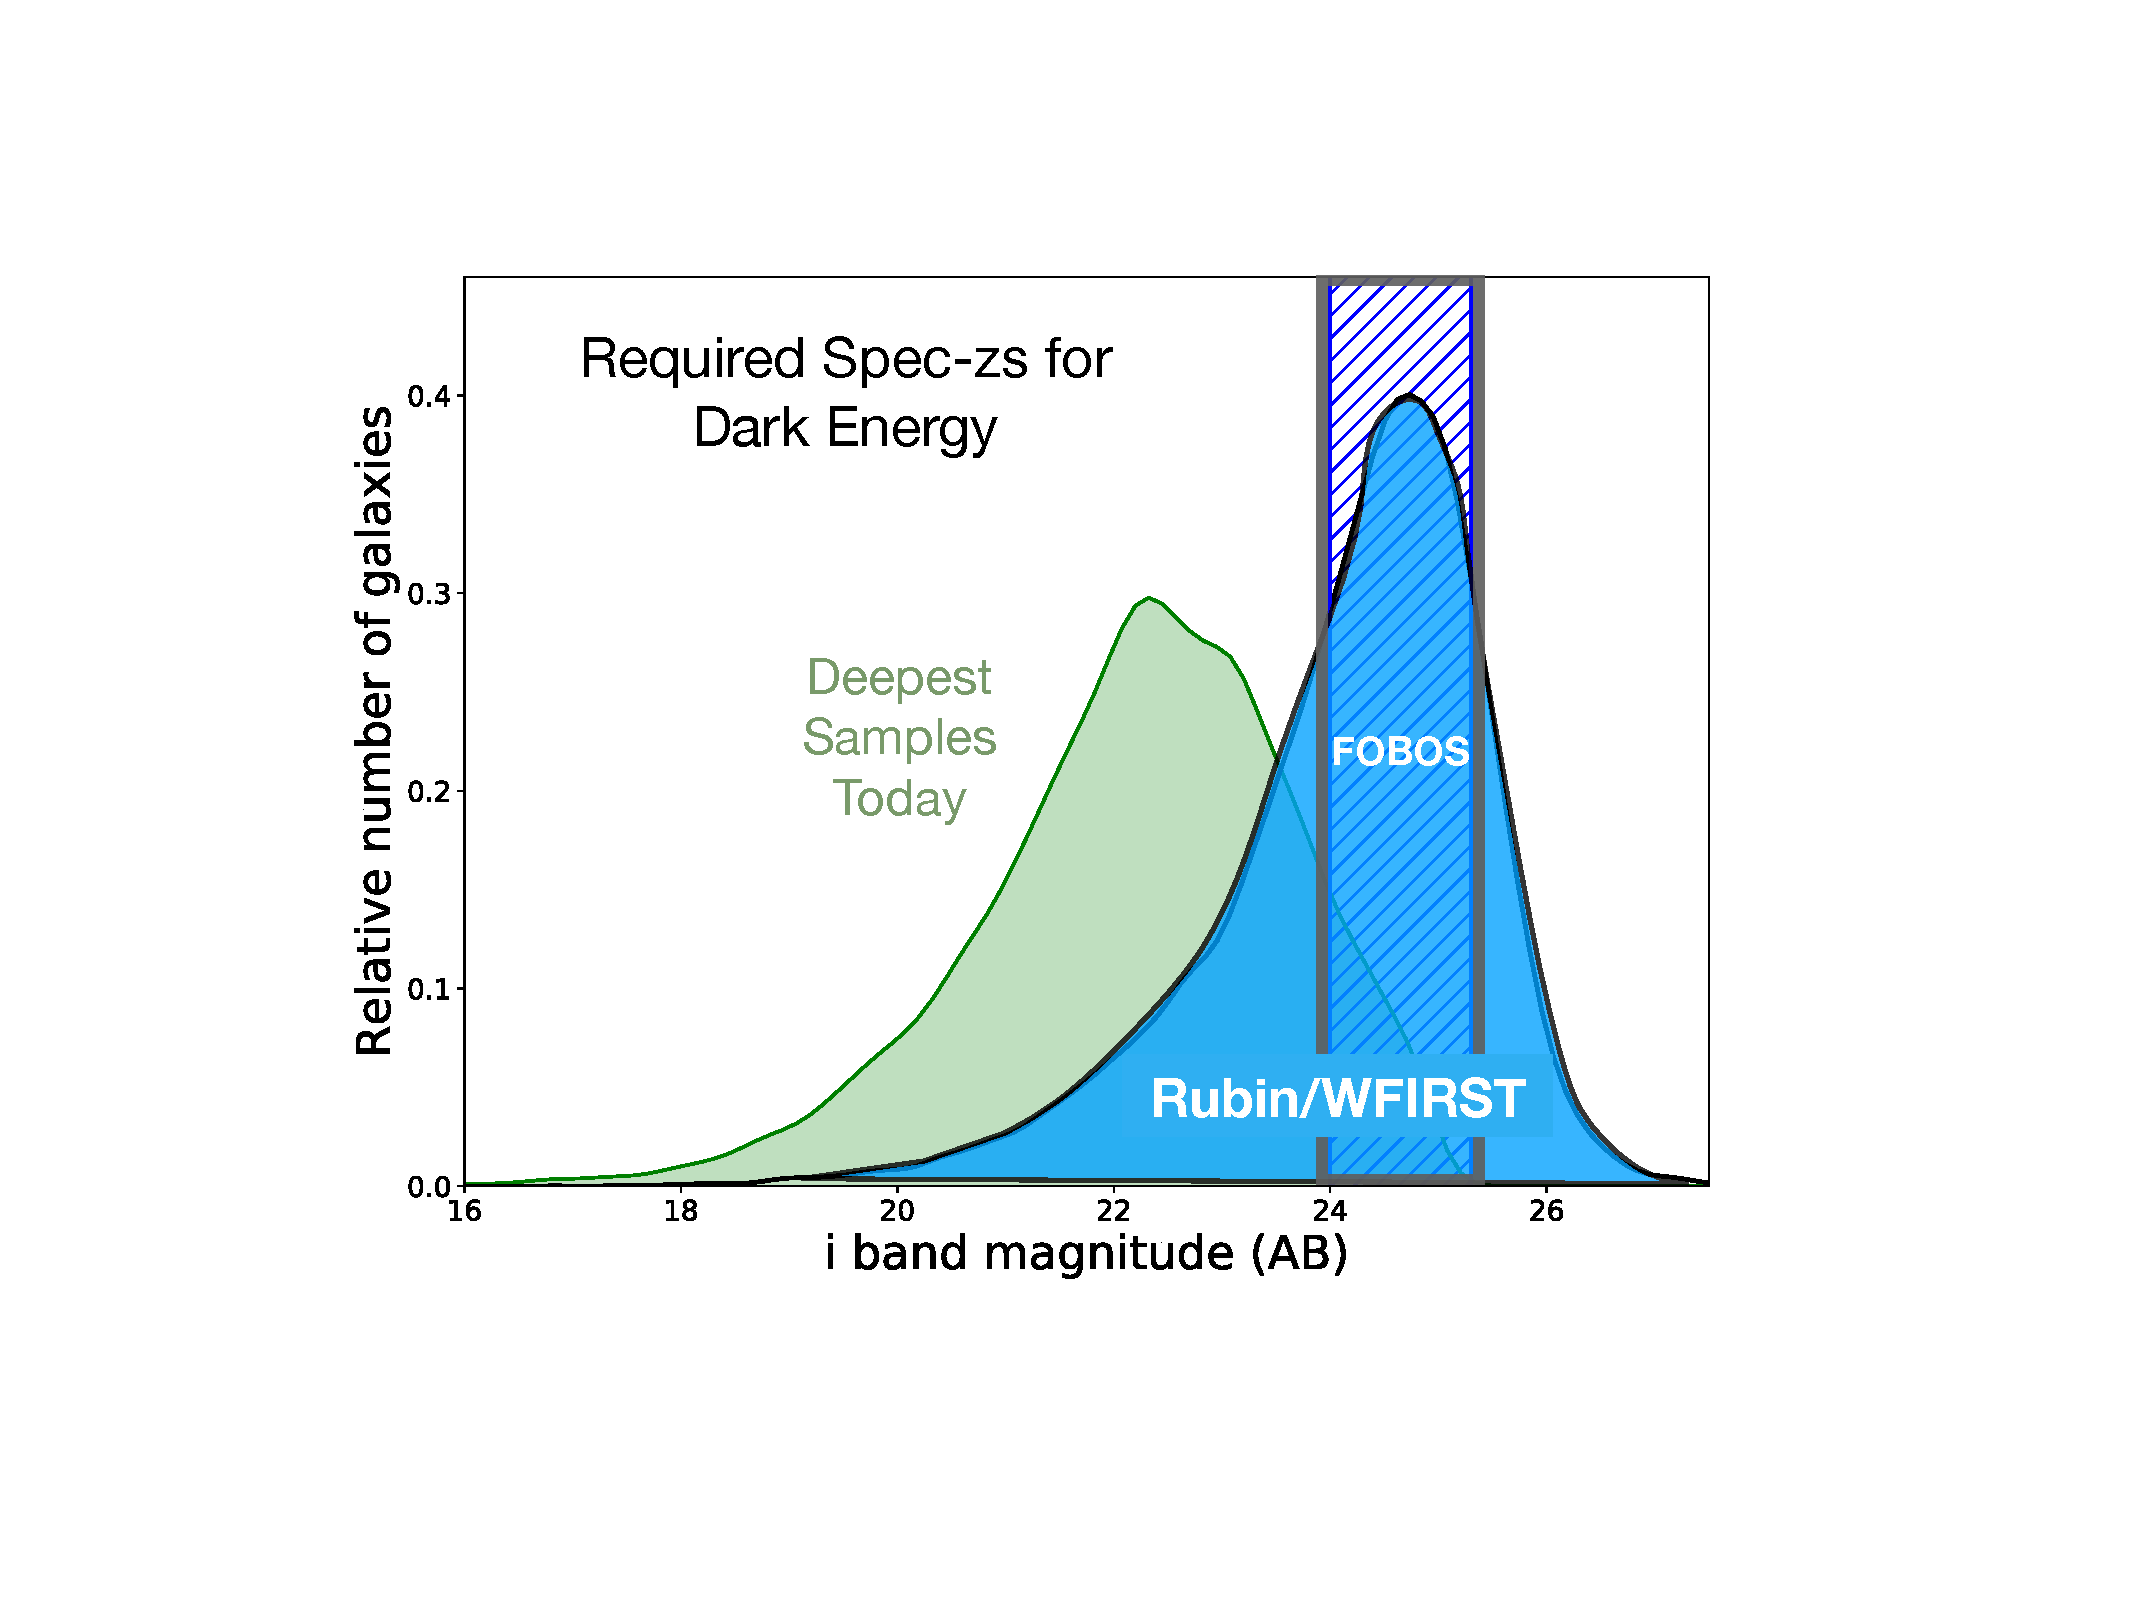
\includegraphics[width=0.5\textwidth]{figs/fobos_cosmology_v2.pdf}
\caption{\footnotesize Magnitude distribution of secure spec-$z$ samples in existing deep fields from, e.g., DEEP2, VVDS, VIPERS, C3R2, and zCOSMOS ({\it green}), compared with an anticipated distribution of the LSST/Roman weak-lensing sample (\textit{blue}) \citep{hemmati18}. Ultra-deep (50hr) exposures in the FOBOS cosmology program are designed to obtain spec-$z$s for $\sim$15k faint galaxies in the hatched region, representing roughly 50\% of the weak-lensing sample of these missions and weakly constrained by current spec-$z$ samples. The FOBOS cosmology program would operate over 12 independent regions to mitigate cosmic variance, employing a careful selection to explore the full color-magnitude parameter space efficiently \citep{masters15}.}
\label{fig:cosmos_magdist}
\end{wrapfigure}

The {\it FOBOS Cosmology Program} will play a critical role by training photo-$z$s from sources with spectral features too blue or fluxes too faint for other instruments, like PFS,\footnote[1]{Subaru's Prime Focus Spectrograph (PFS) commissioning in 2022.} but that dominate by number (Fig.~\ref{fig:cosmos_magdist}).  For example, Rubin Observatory will begin reaching the LSST target 5$\sigma$ point-source depth of $i = 26.8$~(AB) in 2029.   FOBOS spectroscopic follow-up to $i_{AB} = 25.3$ for extended sources will provide a well-matched training sample\footnote[1]{\citet{newman15} emphasize that photo-$z$ ``calibration'' can be accomplished by cross-referencing all-sky surveys of various low-density tracers like quasars and associated absorbers, luminous red galaxies, and emission-line galaxies.} that will \emph{increase LSST's dark energy figure-of-merit by 40\%} \citep{newman15}. No other existing or planned instrument will obtain such a spectroscopic sample on this timescale.  

% Indeed, although Euclid and WFIRST will both perform grism spectroscopy, the relatively low sensitivity and strongly biased samples (e.g., they will be far more sensitive to galaxies with strong emission lines) mean that grism spectra from these missions are insufficient to train photo-$z$s for the full weak-lensing samples.  Additionally, because FOBOS has no ``redshift desert'' (its blue wavelength coverage allows redshift determination at $1.5\lesssim z \lesssim2.5$ via Ly$\alpha$ and/or nearby UV absorption features), the {\it FOBOS Cosmology Program} will reduce the need for expensive, space-based\footnote[1]{Ground-based near-IR spectroscopy is too contaminated by night-sky emission lines to provide spec-$z$s at the required level of completeness \citep{newman15}.} near-IR spectroscopy of galaxies with $z > 1.5$.  Beyond enhancing cosmological analyses, the resulting galaxy sample would have a major impact on galaxy-evolution studies by providing the spectroscopic coverage needed to fully leverage photometry for billions of galaxies (see \S\ref{sec:ML}). 

% \smallskip
% \noindent {\textsf{FOBOS Cosmology Program:}}

\subsubsection{FOBOS Cosmology Program}
Over $\approx$130 nights, this program would observe a set of twelve 0.1 deg$^2$ FOBOS pointings arranged evenly in right ascension and chosen to overlap with the LSST, Euclid, and Roman footprints.  The program satisfies the sample size, field variance, and depth requirements of existing survey designs \citep{newman15} by obtaining ultra-deep 50-hour integrations of $\sim$15,000 sources at $24 < i_{AB} < 25.3$, a magnitude range that covers the majority of LSST/Roman weak-lensing samples.  While near-Poisson performance with such extreme integration times has been demonstrated with fiber spectrographs \citep[e.g.,][]{gu17,childress17}, our team's investigation of critical design factors that enable such performance (Bundy et al., in prep) has defined FOBOS instrument requirements, including a multi-tier calibration system (\S \ref{sec:calib}).  Accounting for expected sensitivity and stability, our exposure-time calculator estimates a continuum S/N$\sim3.5$ ($i$-band) for the faintest sources at these depths, a level known to be sufficient for $>75$\% redshift success \citep[e.g.,][]{Newman13, masters19}. 

% With 1200 single fibers (per pointing) from two of FOBOS's three spectrographs assigned to cosmology program targets, parallel observations with IFUs fed to its 3rd spectrograph can leverage the ultra-deep exposures needed for targets in the {\it FOBOS Galaxy Ecosystem Program} (\S \ref{sec:galaxies}).  Photo-$z$ calibrators targeted by single fibers will efficiently span color-magnitude space \citep{masters15, masters19} with dynamic re-allocation of fibers to new targets as successful redshifts are obtained.  This program would request 12.5 dark nights per year.


%-----------------------------------------------------------------------

%\begin{wrapfigure}{r}{0.6\textwidth}\small
%\vspace{-0.2cm}
\begin{figure}
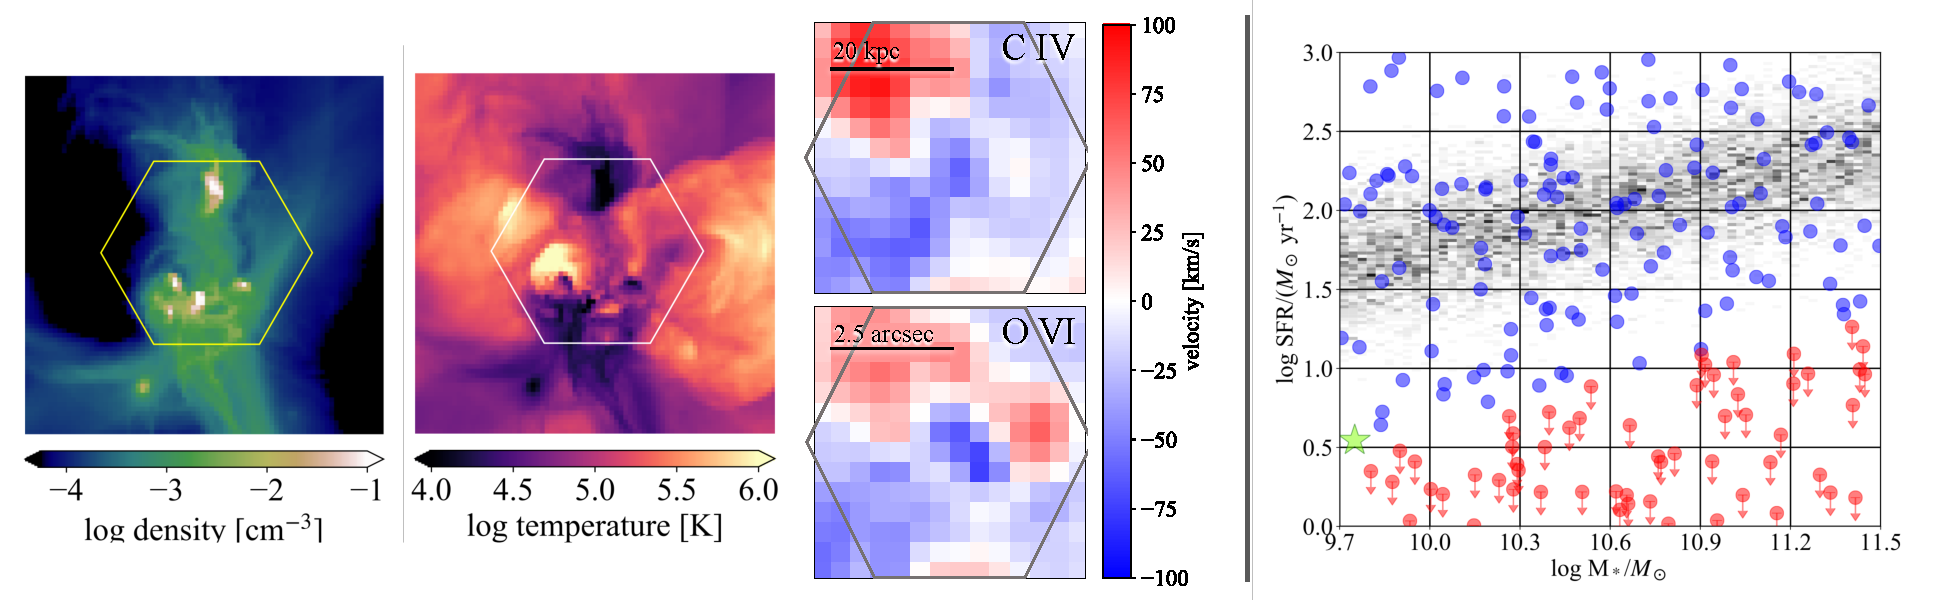
\includegraphics[width=\textwidth]{figs/msipProposalCgmCombo.pdf} %figs/CGMscience_v3.pdf}
\caption{\footnotesize {\it Left}: Simulations of the density and temperature of the CGM at $z=2-2.5$ \citep{Corlies:2018aa}. {\it Center}: Predicted observations of CGM emission sampled by the FOBOS IFUs, providing kinematic maps that trace gas flows using UV tracers (C IV and O VI).  {\it Right}: The {\it FOBOS Galaxy Ecosystem Program} will map these features for hundreds of galaxies sampling a large range physical parameters.  This panel shows a mock sample of program galaxies (star-forming in blue; passive in red) in the stellar mass-star formation rate ($M_*$-SFR) parameter space; the example simulation shown to the left is marked by a green star. The $M_*$-SFR ``main sequence'' \citep{Whitaker:2012} is shown as the underlying gray 2D histogram.}
\label{fig:cgmsample}
\end{figure}
%\end{wrapfigure}

\subsection{Mapping the Baryonic Ecosystem of Early Galaxies at All Scales}
\label{sec:galaxies}

The fueling and regulation of galaxy growth during the peak formation epoch ($z \sim2$--3) is critically tied to the turbulent and gas-rich ecosystem in which early galaxies evolve. The James Webb Space Telescope (JWST) and upcoming extremely large (30m-class) telescopes (ELTs) will marshal powerful infrared observations to study the stars and nebular gas at the heart of these early galaxies. But mapping the large-scale gaseous environments and filamentary networks that fuel and ultimately regulate galaxy evolution at these redshifts requires high multiplex absorption-line tomography and rest-frame UV spectral coverage.  FOBOS enables an ambitious two-prong approach to characterizing galaxy ecosystems on all scales: a detailed tomographic study of the cosmic web at $z>1.5$ combined with an ultra-deep IFU survey of emission from the circumgalactic medium (CGM) of $\sim$180 galaxies at the peak of cosmic star formation.

% As FOBOS comes on-sky, the PFS Strategic Survey Program on Subaru (running 2023--2028) will have completed an important first step in IGM Ly$\alpha$ tomography by making a map of structure at $2.1 < z < 2.5$ over 15 deg$^2$.  This map will be relatively coarse, however, with a sightline density of 1600 deg$^{-2}$.  While it will provide valuable statistical measures of cosmic web structures, a detailed study of the interplay between the fueling and feedback mechanisms mediated by these structures requires chemical and kinematic diagnostics that are only possible with more fine-grain resolution and higher S/N.  

% FOBOS, with its high sampling density, sensitivity, and blue wavelength coverage, will provide these diagnostics via follow-up of high-value regions in the PFS IGM map, such as protoclusters and galaxy overdensities, increasing the source density over PFS by a factor of 4--10 (depending on location).  This higher density yields statistical insight at 1 Mpc separations (the scale of individual massive halos) and the ability to stack sightlines to gain further in S/N so that various heavy-element ion transitions can be studied.  FOBOS will also be able to extend tomographic reconstruction down to $z = 1.5$, where sources are brighter.

%(\S \ref{sec:landscape})

FOBOS's unique UV sensitivity and IFU capabilities will deliver the first significant samples of high-$z$ galaxies with circumgalactic gas mapped \emph{in emission}. UV sensitivity opens access to high- and intermediate-ionization transitions, such as O VI ($\lambda_{\rm rest} = 1032, 1037$ \AA) and C IV ($\lambda_{\rm rest} = 1548, 1550$ \AA), which probe $10^{5-6}$ K and $10^4$ K gas, respectively.  The combination of single-fiber and multiplexed IFU observations therefore allows FOBOS to map the density and dynamical state of diffuse gas at all relevant scales from the IGM to the CGM, providing novel constraints on the next generation of cosmological simulations.

% This temperature range marks the peak in gas cooling and therefore constrains how gas rains onto galaxies to fuel star-formation, as well as tracks feedback processes that establish and regulate the CGM (Fig.~\ref{fig:cgmsample}).  While $z\sim2$ galaxy halos may be mapped in Ly$\alpha$ on a one-by-one basis with KCWI (and metal-line emission has already been studied in some extreme objects), FOBOS will map these diagnostics to greater depth and for a large sample of ``normal'' galaxies (Fig.~\ref{fig:cgmsample}).  The combination of single-fiber and multiplexed IFU observations therefore allows FOBOS to map the density and dynamical state of diffuse gas at all relevant scales from the IGM to the CGM, providing novel constraints on the next generation of cosmological simulations.

% In longer term, think through science that we should be proposing now-ish to do with JWST with the idea that we can follow-up with FOBOS.

% Billion galaxy survey?
%Field selection will take advantage of quasar-quasar pairs 
%at \note{range or exact number?} certain redshifts.

\subsubsection{FOBOS Galaxy Ecosystem Program}

The two observing campaigns of the {\it FOBOS Galaxy Ecosystem Program} would link the buildup of the CGM to the cosmic web (IGM): (1) The IGM tomography component would span a total of 6 deg$^2$, delivering fine-sampling and detailed follow-up of cosmic structures identified in the PFS IGM maps.  With a 3-hour integration time, the program targets over 1000 background Lyman-break galaxies per FOBOS pointing (60,000 total), obtaining ${\rm S/N} \sim 3.5$ at $r_{AB} \approx 24.6$, which is sufficient for building a dense network of Ly-$\alpha$ absorbers associated with targeted structures at $z = 1.5$--2.5 \citep{lee16}. An additional $\sim$600 fibers per pointing will be allocated to galaxies embedded in the cosmic web. Executing this component would require 18 nights.  (2) In a joint observing scheme with the ultra-deep exposures of the {\it FOBOS Cosmology Program}, the CGM study would use FOBOS's unique IFU multiplex capability (configuring one-third of FOBOS's fiber complement into into 15 37-fiber IFUs) to build an unprecedented sample of galaxies spanning respectively $\sim2$ and $>3$ orders of magnitude in $M_\ast$ and SFR, with maps of their CGM {\it in emission}.  Each IFU will observe an on-sky diameter of 5.6 arcsec, sampling gaseous halos in each galaxy at 5 kpc scales out to a radius of 20--25 kpc (Fig.~\ref{fig:cgmsample}).  These observations require the equivalent of 12.5 dark nights per year.

%{Baseline source density goals for PFS: 1600/deg$^2$ over 15 deg$^2$.  This sightline density translates to 100 sources over the FOBOS FOV.  From the luminosity function of LBGs, going to a depth of R = 24.5 affords 400 possible $z=2.0-3.0$ sources within a single FOBOS pointing.  A 3-hr observation delivers S/N$\sim4$ per pixel in the g band.  Going to R = 24.6 means 1000 possible sources per FOV at S/N$\sim3.5$.  If we improve on source density over PFS by a factor of 4, we reduce the average sightline separation to $\sim1$ per comoving Mpc, or resolving scales of most massive individual halos!  This leaves 1400 fibers for `embedded' galaxies in the foreground. }

% \note{Joe/Dan/Kyle: play-out the combination of the 2nd program above and the Cosmology program as a practical illustration of what a series of observing nights devoted to these programs might look like. }

\subsection{Discovery in the Time Domain}
\label{sec:kilonovae} 

% The joint detection of electromagnetic radiation and gravitational waves from GW170817 began a new era of multimessenger astronomy.  This single binary neutron star merger and its associated kilonova has remade our understanding of multiple branches of astrophysics, from the physical nature of mergers and explosion mechanisms to the origin of the heaviest elements in the universe.  

Once FOBOS goes on-sky in the late 2020s, gravitational wave detectors like LIGO,\footnote[1]{The Laser Interferometer Gravitational-Wave Observatory} Virgo and KAGRA\footnote[1]{The Kamioka Gravitational Wave Detector, formerly the Large Scale Cryogenic Gravitational Wave Telescope (LCGT)} will routinely detect $\sim$30 binary neutron star mergers with kilonovae (KNe) annually \citep{abbott2018prospects}, providing the samples needed to understand how the physical properties and nucleosynthetic yields of KNe vary with environment.  FOBOS will be crucial to obtaining rapid spectroscopy of the Lanthanide-free ``blu'' component of the KN light curve, which peaks within a day post-merger at $\lam_\mathrm{peak}\sim0.35$ $\mu$m (Fig.~\ref{fig:kilonova}). When deployed as the Keck II instrument, FOBOS's always-ready IFU makes it ideal for instant target acquisition and host galaxy characterization, all while simultaneously observing serendipitous targets of interest in the same field-of-view. 

%, each with a typical localization region of $\Omega_\mathrm{90\%}<100$ deg$^2$ . 

FOBOS follow-up will trigger on Rubin target-of-opportunity observations, which will search for KNe within an hour after the gravitational wave alerts are issued \citep[assuming the strategy proposed by][]{margutti2018}. For a typical 50 deg$^2$ localization region, we expect $\sim$100 KN candidates with $m_i\lesssim22.5$, the expected KN brightness at a sensitivity distance of 200 Mpc \citep{cowperthwaite2017, goldstein2019}.  Indeed, beyond KNe, Rubin Observatory will discover well over 1 million extragalactic transients annually, including thousands of currently-rare sources such as tidal-disruption events \citep{bricman2020}, superluminous supernovae \citep{villar2018} and changing-look quasars. Nearly every FOBOS pointing will contain $\sim$5 LSST transient hosts.  The {\it FOBOS Time-Domain Program} will include a large-scale environmental study of such transients by allocating free fibers from other ongoing programs to those targets.

% Identifying and triggering spectroscopic investigations of the true KN will require FOBOS's rapid and blue-sensitive follow-up capabilities.  By deploying the remaining single fibers and IFUs on separate, pre-assigned transient sources in each pointing, we will take maximum advantage of synergies with time-series data from the world-wide follow-up observations of these gravitational-wave fields. 

% \begin{wrapfigure}{r}{0.6\textwidth}%\small
\begin{figure}
\centering
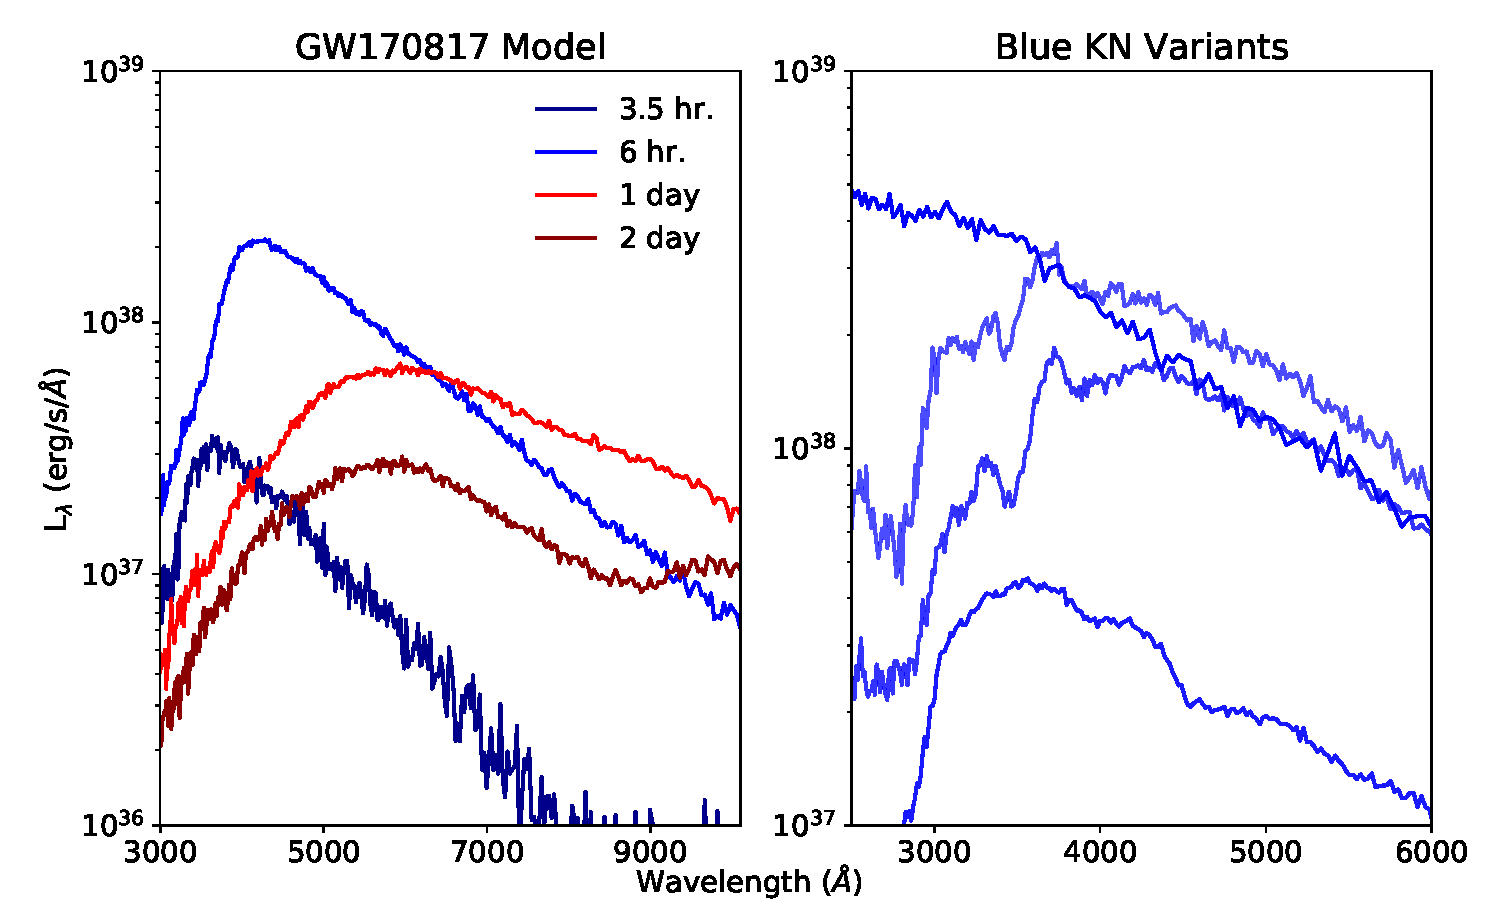
\includegraphics[width=0.7\textwidth]{figs/kn_fobos.pdf}
\caption{\textit{Left:} Model kilonova spectra \citep{kasen2017} based on GW170817 taken 3.5 hours, 6 hours, 1 day and 2 days post-merger. \textit{Right:} Variations of ``blue" kilonovae, generated by varying the energy, mass and Lanthanide fraction of kilonova models. FOBOS's blue sensitivity is essential to discriminate between these early-time models.}
\label{fig:kilonova}
\end{figure}

  % Through coordination with {\it FOBOS Cosmology} and {\it Galaxy Ecosystem Programs}, we will also target transients with FOBOS IFUs, dramatically increasing resolved spectroscopy of extragalactic hosts \citep[see a recent review by][]{anderson2015} at little additional cost. 


% \noindent {\textsf{FOBOS Time Domain Program:}}

\subsubsection{FOBOS Time-Domain Program}

Via rapid follow-up of KN candidates discovered by LSST, FOBOS can undertake a systematic population study of KNe and their environments. We expect $\sim4$ KNe to be detectable by LSST and FOBOS annually. For each triggered event, we would target up to $\sim50$ candidates with 10-min observations per event over two nights, nearly twice the total spectroscopic follow-up effort currently possible \citep{hosseinzadeh2019}. We would observe each candidate with FOBOS's central, fixed IFU to obtain a redshift and potential-host properties.  If our monitoring of real-time quick-look reductions identifies the KN, our strategy would immediately initiate deeper ($\sim1$ hour) observations to potentially capture ``blue'' kilonovae (Fig.~\ref{fig:kilonova}).  With four KNe annually, this FOBOS program requires $2.5$ nights per year; beyond the KNe observations, many fibers would be allocated to pre-assigned transient sources.

% Additionally, FOBOS would observe active transients in pointings from the {\it FOBOS Cosmology} and {\it Galaxy-Ecosystem Programs}.  In the $\sim$24 pointings that overlap with LSST Deep Drilling Fields, we expect $\sim$150 total transients to be visible each year with $m_i<24$. We assign a single IFU to simultaneously observe the transients and their host galaxies (at $z<1$). FOBOS's blue sensitivity will be especially valuable for shock-driven (e.g., Type IIn supernovae) and relativistic events \citep[e.g., the atypically bright Type Ib supernova AT 2018cow;][]{margutti2019}, which peak near $\sim$0.3~$\mu$m. 


%small calculations: passing a KN spectrum through the obs calc, we need ~10 min exposures for m  = 22.5 events, leading to roughly 3.5 hrs in a ToO night



%-----------------------------------------------------------------------

% \begin{wrapfigure}{r}{0.58\textwidth}%\small
\begin{figure}
\centering
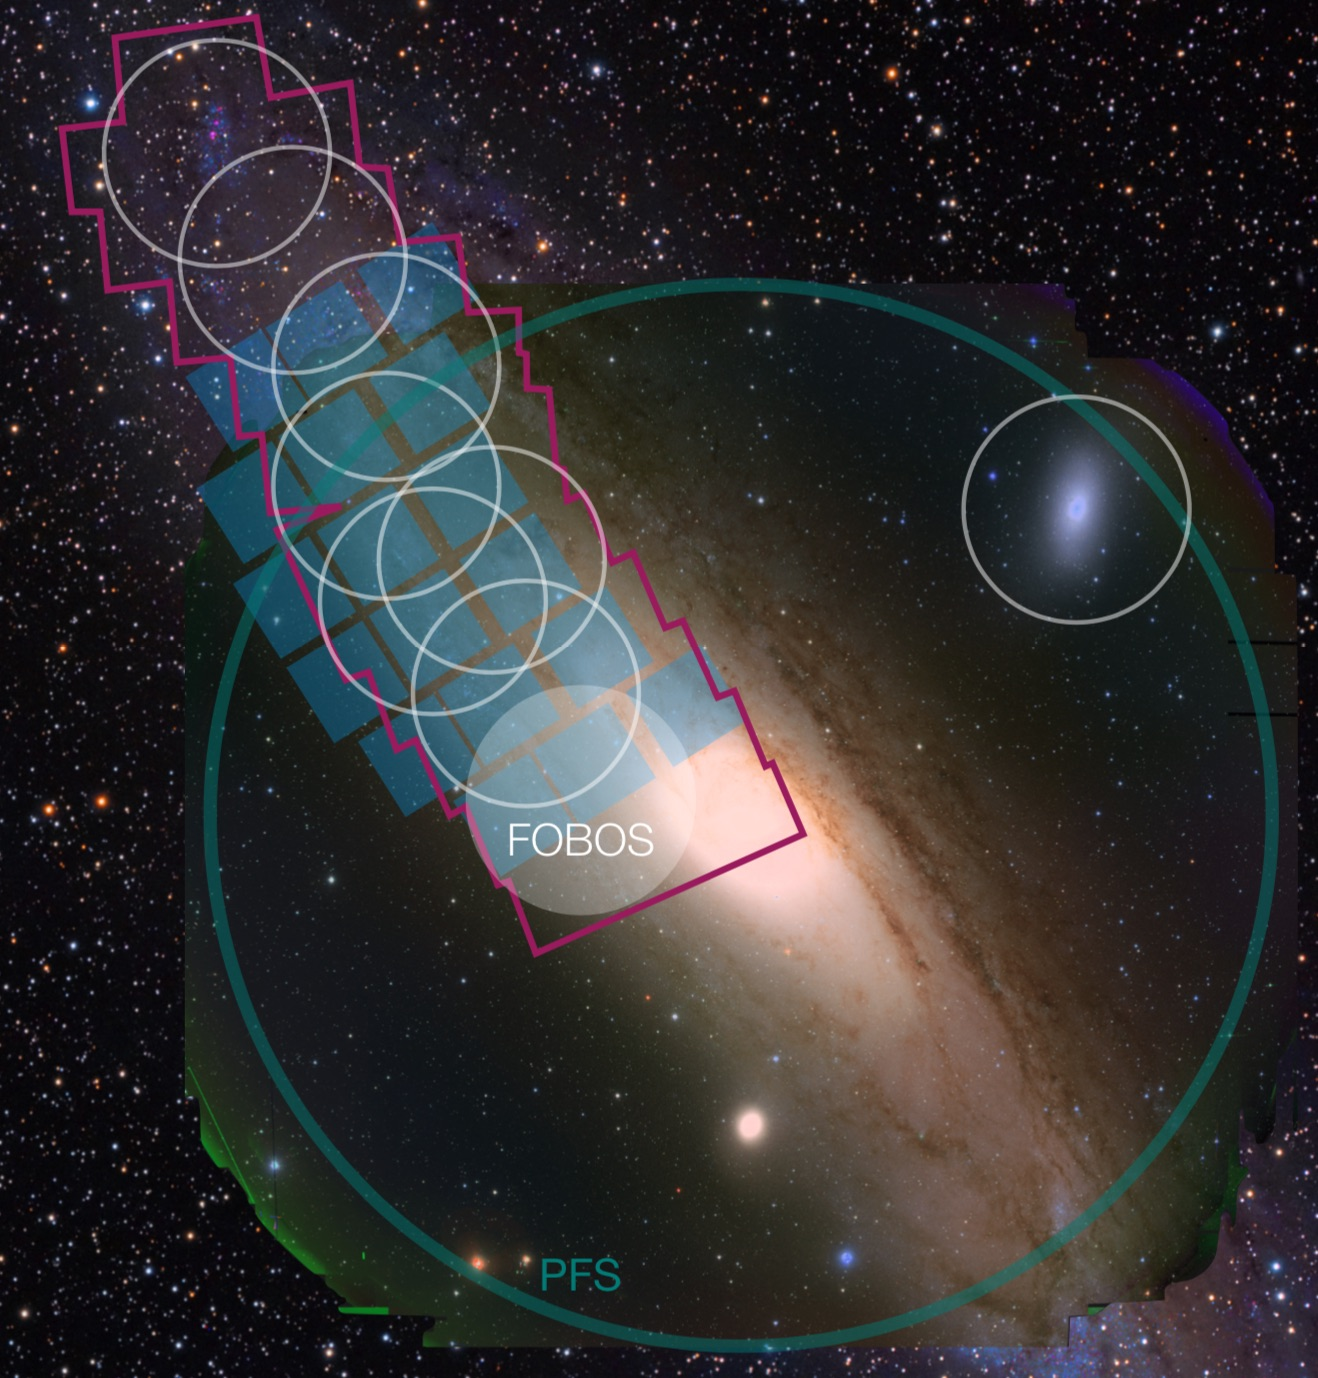
\includegraphics[width=0.55\textwidth]{figs/M31_footprint_v3.jpg}
\caption{A Subaru HSC image (lower right) superposed on a larger background image of M31 (credit: Adam Evans).  FOBOS pointings (white circles) span the PHAT area (magenta) and NGC 205.  The Subaru-PFS FOV (green circle; similar to MSE) and single-pointing Roman imaging footprint (blue squares) are also shown.}
\label{fig:M31}    
\end{figure}

\subsection{Assembly and Evolution of Andromeda's Disk and Satellite Galaxies}
\label{sec:localgroup}

Galaxy groups like the Local Group, with two L$^*$ galaxies, dominate the nearby universe \citep{kourkchi17}.  We expect galaxies in such groups to share common assembly histories, and yet, the Milky Way and Andromeda galaxies appear to have evolved in significantly divergent ways.  Differences from their star-cluster populations to their dwarf-galaxy properties remain poorly understood, limiting progress towards building a complete picture for how the Local Group formed and evolved.  

% For the Milky Way, stellar properties (e.g., age, metallicity, $\alpha$ abundance) and kinematics from large-scale spectroscopic surveys (e.g., APOGEE, GALAH, LAMOST) are now being combined with exquisite astrometric data from {\it Gaia} to provide a revolutionary view of its evolution.  For example, these data reveal a clear bimodality in $\alpha$ abundance, indicating that stars at relatively greater distances from the disk plane (i.e., ``thick-disk'' stars) were formed in environments with much shorter star-formation timescales, likely due to a merger event that truncated star formation for a time.  Isolating chemically similar groups of stars in this way to reveal their common structural and dynamical properties is now fundamental to our understanding of the Milky Way.  This ``chemical tagging'' offers greater insights than studies of stars selected by their structural or dynamical associations alone.  With FOBOS, we can apply similar methods to the study of M31 and its satellite galaxies.

% Although chemical tagging with M31 benefits from our outside view of this galaxy (compared to our inside view of the Milky Way), it also faces the challenge of obtaining precise stellar parameter measurements for very large samples.  First steps were made by SPLASH\footnote[1]{Spectroscopic and Photometric Landscape of Andromeda’s Stellar Halo \citep[e.g.][]{splash}} which obtained $\sim$1hr Keck-DEIMOS exposures for $\sim$10,000 RGB stars in the disk, stellar streams, and halo of M31.  \citet{dorman15} used SPLASH to study the stellar age and velocity dispersion of disk stars and found that M31 features a much thicker, high-dispersion component than the Milky Way.  More recently, \citet{Escala20} explored metallicity and $\alpha$ abundance trends in 70 RGB stars ($\sim$6hr Keck-DEIMOS integrations) in the outer disk, inner halo, and Giant Stellar Stream of M31.  These trends also suggest a significant, merger-induced star-formation event in M31.  However, without more precise stellar parameters and larger samples --- beyond the limits of what one can expect to achieve with DEIMOS --- clear inferences that contrast the evolutionary histories of the Milky Way and M31 disks are out of reach.

\begin{figure}
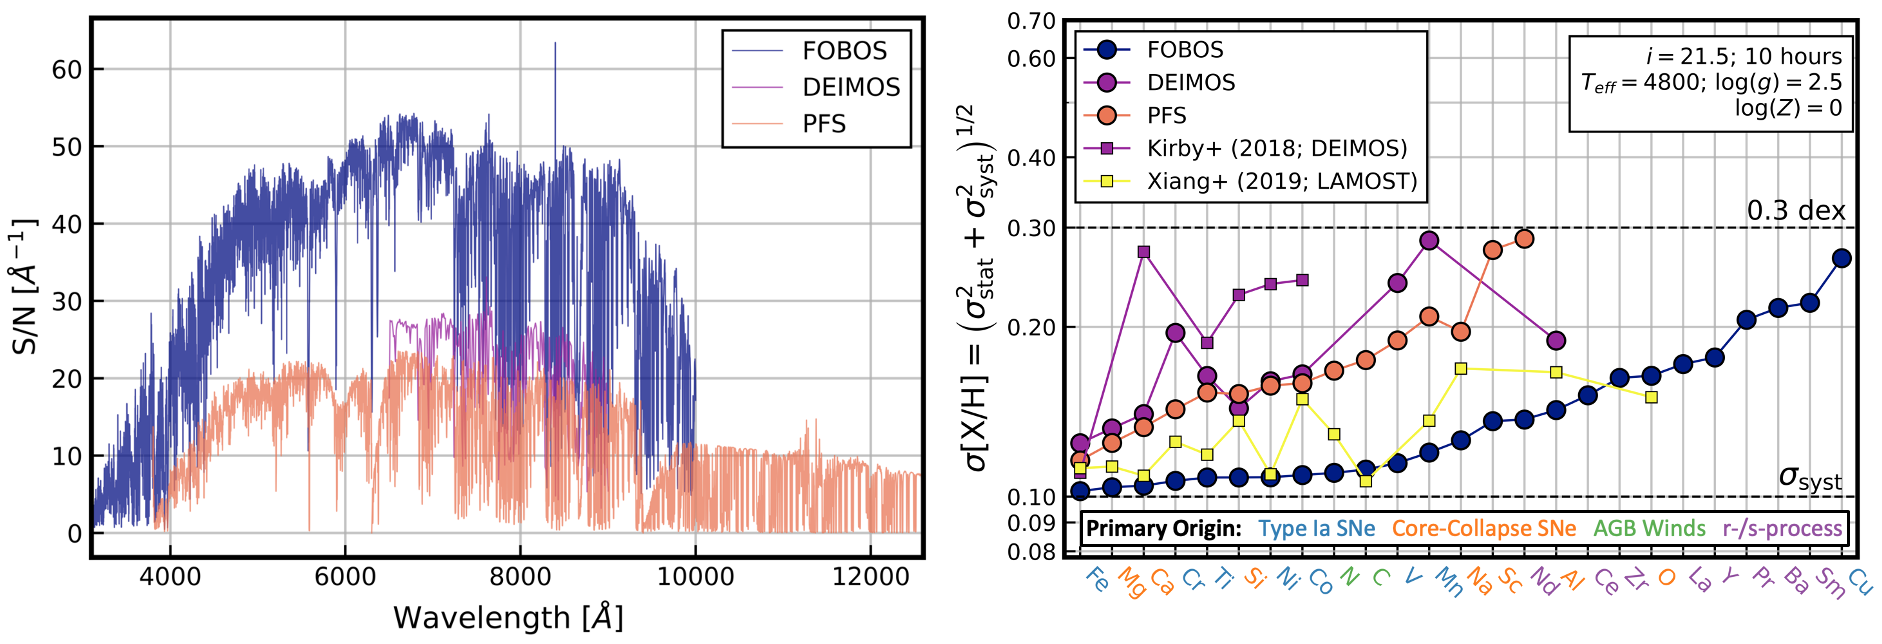
\includegraphics[width=1.0\textwidth]{figs/abundances_snr_v6.png}
\caption{Simulated observations demonstrating FOBOS's ability to perform ``chemical tagging'' in M31 and M33. \textit{Left:} Expected S/N for an $i=21.5$ RGB star in M31 observed for 10hr using FOBOS, PFS, and DEIMOS. \textit{Right:}  Forecasted abundance precision for these observations (filled circles), including both statistical uncertainty ($\sigma_{\rm stat}$; predicted by the Cram\'er-Rao Lower Bound) and a 0.1-dex systematic uncertainty \citep[$\sigma_{\rm syst}$; cf.,][]{kirby18, Xiang2019}. Elements are ordered along the ordinate by decreasing precision (limited to $\lesssim$0.3 dex) and color-coded by their primary nucleosynthetic origin. Although these forecasts are optimistic, the indicated \textit{relative} precision between instruments is robust. Direct abundance uncertainties \citep[][purple squares]{kirby18} from DEIMOS spectra of $-1.0<\text{[Fe/H]}<-0.6$ RGB stars in MW satellites with comparable S/N to our simulations are shown for reference; their measurement precision is worse than our DEIMOS predictions primarily because of their lower metallicity targets.  We also show abundance uncertainties from LAMOST spectra of MW RGB stars \citep[][yellow squares]{Xiang2019}, scaled to the S/N and resolution of the proposed FOBOS observations.}
\label{fig:abundances_snr}
\end{figure}

The {\it FOBOS Andromeda Program} would deploy ``chemical tagging'' techniques to the disk of M31, building a sample that is both 10 times larger than previous efforts and significantly deeper.  With FOBOS's wavelength coverage and sensitivity, we will measure precise velocities ($<$ 1 km/s), [Fe/H] and [$\alpha$/Fe] to $\sim$0.1 dex, individual elemental abundances to $\lesssim$0.2 dex \citep[Fig.~\ref{fig:abundances_snr}; cf.][]{YST2017}, and stellar age from blue CN absorption features.  Complementing the upcoming wide-field ($\sim$20 kpc at M31 distances) mapping of the M31 halo with PFS and MSE,\footnote[1]{The Maunakea Spectroscopic Explorer (MSE) is a concept being developed for a future telescope and instrument at the current Canada-France-Hawaii Telescope site.} these data will provide the first clear, spatially-resolved measurements of chemodynamical trends in M31's disk, allowing us to address two key questions for the first time: Does M31, like the Milky Way, exhibit its own [$\alpha$/Fe] bimodality?  If so, were the ancient merger histories of the two galaxies linked or largely independent?

The program also includes campaigns of 500 young stellar clusters in M31's disk \citep[dwarfing even Milky Way samples,][]{johnson15}, the dense cores of M31's major galaxy satellites, and 10,000 RGB stars in M33's disk.  In particular, observations of young stellar clusters capitalize on FOBOS's blue sensitivity and IFU capabilities.

\subsubsection{FOBOS Andromeda Program} The program is designed in two parts. (1) We would construct benchmark spectroscopic samples of 100,000 and 10,000 RGB stars in the disks of M31 and M33, respectively.  We target six M31 pointings in the PHAT\footnote[1]{Panchromatic Hubble Andromeda Treasury \citep{phat}} region between 5--20 kpc.  Each pointing is visited 10 times, and two disk pointings beyond 20 kpc are each visited once.  In M33, we target 3 pointings, each visited twice.  Each visit will target a unique set of stars with a total integration time of 10 hours, delivering $i$-band ${\rm S/N} \approx 40$ \AA$^{-1}$ and $\approx 20$ \AA$^{-1}$ at the  ``sweet-spot'' of the RGB ($i_{Vega} = 21.5$) and a magnitude fainter, respectively.  This ensures a radial-velocity precision of $<$1 km/s {\it for all targets} and precise metallicity and abundance measurements, as illustrated in Fig.~\ref{fig:abundances_snr}.

% Accounting for a 60\% rejection rate \citep{dorman12} due to crowding of ground-based RGB catalogs ($i_{\rm Vega} < 22.5$), we target six M31 pointings in the PHAT\footnote[1]{Panchromatic Hubble Andromeda Treasury \citep{phat} is a multi-cycle HST program that maps $\sim1/3$ M31's star-forming disk in 6 filters.} region between 5--20 kpc.  Each pointing is visited 10 times, and two disk pointings beyond 20 kpc are each visited once.  In M33, we target 3 pointings, each visited twice.  Each visit will target a unique set of stars --- the stellar density is high enough to efficiently target new stars for each visit with $\sim$95\% completeness --- for a total integration time of 10 hours, an order-of-magnitude longer than the SPLASH survey.  We expect $i$-band ${\rm S/N} \approx 40$ \AA$^{-1}$ and $\approx 20$ \AA$^{-1}$ at the  ``sweet-spot'' of the RGB ($i_{Vega} = 21.5$) and a magnitude fainter, respectively.  This ensures a radial-velocity precision of $<$1 km/s {\it for all targets} and precise metallicity and abundance measurements, as illustrated in Fig.~\ref{fig:abundances_snr}.
%an internal [Fe/H] precision between 0.05 and 0.1 dex, and an internal [$\alpha$/Fe] precision of 0.1 dex for all spectra with ${\rm S/N} \geq 20$ \AA$^{-1}$. For many stars, individual iron-peak and $\alpha$ elements, as well as C and N, will also be measurable to $\lesssim 0.2$ dex. 
% This combination of sample size and precision allows us to directly compare radial trends in chemodynamical structures between M31, M33, and the MW. (2) Jointly with single-fiber observations of RGB stars, we would acquire IFU observations ($\sim$5.6\arcsec{} diameter) of $\sim$500 young star clusters in the M31 disk.  It would also dedicate 3 pointings (each visited once) for MOS observations of RGB stars in the area including NGC 147, NGC 185, and And II, and use a single pointing (visited twice) for NGC 205.  These observations target 9,000 RGB stars in the central regions of Andromeda's major satellites, yielding their dynamical masses, star-formation histories, and chemical composition.  The two components of the {\it FOBOS Andromeda Program} would require a total of 19 nights per year over 5 years. 

% FROM THE PEP: Do we want to add this back in as a science case for the IFU:  Additionally, a few large-scale star-formation complexes are observed with FOBOS's monolithic IFU (FOV ~700 arcmin2) allow for comparison of the local star-formation activity with the Milky Way. 

% SPECTRAL RANGE BENEFITS OF FOBOS.  INTEGRATE THIS INTO THE TEXT?
% \note{YST: Depending on the stellar type: oxygen information: direct information is possible for M-giant, but not for K-giant, for the latter, it can be nonetheless be inferred using CNO balance in CN and CH bands. On measuring oxygen in the optical, see Fig 2 https://arxiv.org/abs/1801.07370. Nathan: Including wavelengths below 4000 \AA\ makes the most difference to measuring C, N, and O b/c of the CN and CH bands as Yuan-Sen mentioned. There are some Ni and Cu lines that are gained as well, but the precision of most other abundances don't benefit significantly from the bluer wavelength coverage (probably b/c of the lower S/N in the blue).}

% KBW: Integrate more of what's below into the text?

% \note{Yuan-Sen: Maybe a sentence summarizing the importance of alpha vs Fe? E.g., looking for disrupted satellites, reconstruction SFH / satellite mass function through chemical evolutionary tracks.}

% Indeed, FOBOS will provide high-S/N stellar spectra that connect [Fe/H] and [$\alpha$/Fe] patterns to the underlying dynamics, as well as integral-field observations of young stellar clusters  to determine their present-day mass function \note{ref}.  Combining these FOBOS observations with integral-field data from the SDSS-V Local Volume Mapper
%\note{Yuan-Sen: LVM is on the Milky Way though; Kyle: Did the scope of LVM change?  I thought it was going to include maps of local (group) galaxies, as well?}
% and PFS/MSE surveys of halo structure, a complete picture of the Andromeda system's formation history will address key questions about disk evolution, radial migration, dwarf satellites, and dark matter substructure with a level of statistical power that has so far been limited to the Milky Way. Empirical assessments of these phenomena are critical tests for numerical simulations of the formation of the Local Group.


%\note{Yuan-Sen: since the last proposal, the paper about measuring abundances at R~2000, S/N=30 (per pixel) spectra is now published. https://arxiv.org/abs/1908.09727 . I remain rather optimistic that we can measure multiple elements including s-process from these spectra.}


% KBW: Add this into the discussion?
%\note{Nathan: I agree w/ Yuan-Sen, I think we're underselling the abundance measurements these observations will enable. Even at the lower S/N end we should be able to measure more than just Fe and alpha. At the higher S/N end we might expect to measure a few neutron-capture elements (including Ce, Zr, La, Y, and Ba). I can provide plots for reference, even if not for inclusion in the proposal.}

%\note{Mike R.: Pandas link; structures revealed because of increased depth, target densities; luminosity function of red giants}

% This needs a better title...
\subsection{Breadth of Additional Science through Interleaved Programs}
\label{sec:addsci}

Beyond the scope of our design-reference key programs, {\bf FOBOS enables a broad range of observations} as a general-purpose facility spectrograph.  Based on interests within our science team, a glimpse of additional FOBOS science includes: Milky Way and M31 halo stars and stellar streams; the Milky Way bulge and globular clusters; newly identified variable stars from cadenced LSST imaging; white dwarfs toward the faint end of the cooling sequence; dwarf-galaxy stellar populations and dynamics; the environments and spectra of sources producing fast-radio bursts;  the structure and dynamics of Coma and Virgo galaxies using globular-cluster and planetary nebulae (PNe) tracers; the kinematics and physical properties of gaseous winds expelled from galaxies; 2D emission-line kinematics and radial trends in stellar-population parameters from stacked spectra in galaxies up to $z \sim 1$; environmental metrics for groups and clusters at $z \sim 1$--2; galaxy cluster and proto-cluster dynamics; QSO light echos in the IGM; black-hole reverberation mapping; and the redshift calibration of LBG samples at $z = 1.5$--5 for CMB lensing cross-correlation.

% These programs all take advantage of FOBOS's capabilities in different ways; however, they collectively benefit from FOBOS's flexible focal-plane sampling with a uniform spectral format.  While maintaining the important freedom of a PI-led observing mode, these design elements also facilitate new synergistic observing modes that capitalize on FOBOS's information gathering power (Fig.~\ref{fig:info}).  Indeed, the high density of future source catalogs ($\sim$40 arcmin$^{-2}$ at $i_{\rm AB} = 25$) in the era of deep-wide imaging allows FOBOS, with a single-fiber density of $\sim$6 per arcmin$^{2}$, to combine multiple programs that target varied source types and disparate science goals at virtually any accessible field location.  A specific example is the joint observations performed by the {\it FOBOS Cosmology} and {\it Galaxy-Ecosystem Programs} (Table~\ref{tab:progreq}).  In a mode where multiple programs acquire spectra in the same field, we can apportion FOBOS usage in units of ``fiber-hours,'' instead of nights, in a way that maximizes observing efficiency.  In particular, this grows the scientific pie by enabling even small programs with rare targets in the ``long tail'' of the target-density distribution to be combined with other, high-density programs.  This concept is critical to the {\it FOBOS Time-Domain Program}, for example.  Accounting for observing time through fiber-hours also broadens FOBOS access by allowing for a continuous allocation of FOBOS fibers to the full U.S.\ community (\S \ref{sec:community}).

%The range of possible science investigations beyond the key programs impressive:
% \note{Kevin/Kyle: expand on the above: provide better definition of "fiber-hour", highlight the research done by they CMU sub-award for MAISTRO; mixing programs benefits from a fixed spectral format, or push this to section 2?}

% \note{Mike R.: Describe an example, "PI-led" MW bulge program that you might want to do with FOBOS?  RR Lyrae?}

% \note{All: It might be useful to have a couple "PI-led" example programs.  Any takers?}

% \note{Kevin/Kyle: Possibly rename this section based on the input and change in content.}

% \note{Dan/All: Add a couple sentences/paragraph describing overlap with LSST, Euclid, WFIRST.}

% \note{Yuan-Sen: on giving a specific example of PI-led projects, I think the bulge/inner galaxy in the blue with GLAO will be amazing. The AO capability is one of the stronger sells, but it is not mentioned much in the current designated cases. If we are willing to sell the idea that we could get multiple elemental abundances of stars too, that will be a game changer. Most inner galaxy studies were done in the red/IR - not much elemental abundance information. The dynamical time in the inner Milky Way is short, so chemistry is crucial to sort things out.}

% \note{Yuan-Sen: Probably already too much, but these spectroscopic sample will also serve as a training set to derive photometric propoerties (metallicity) of stars, similar to photo-z.}

% \medskip

% \begin{figure}[h!]
% % \captionof{table}{Summary of FOBOS Design-Reference Program Concepts}
% 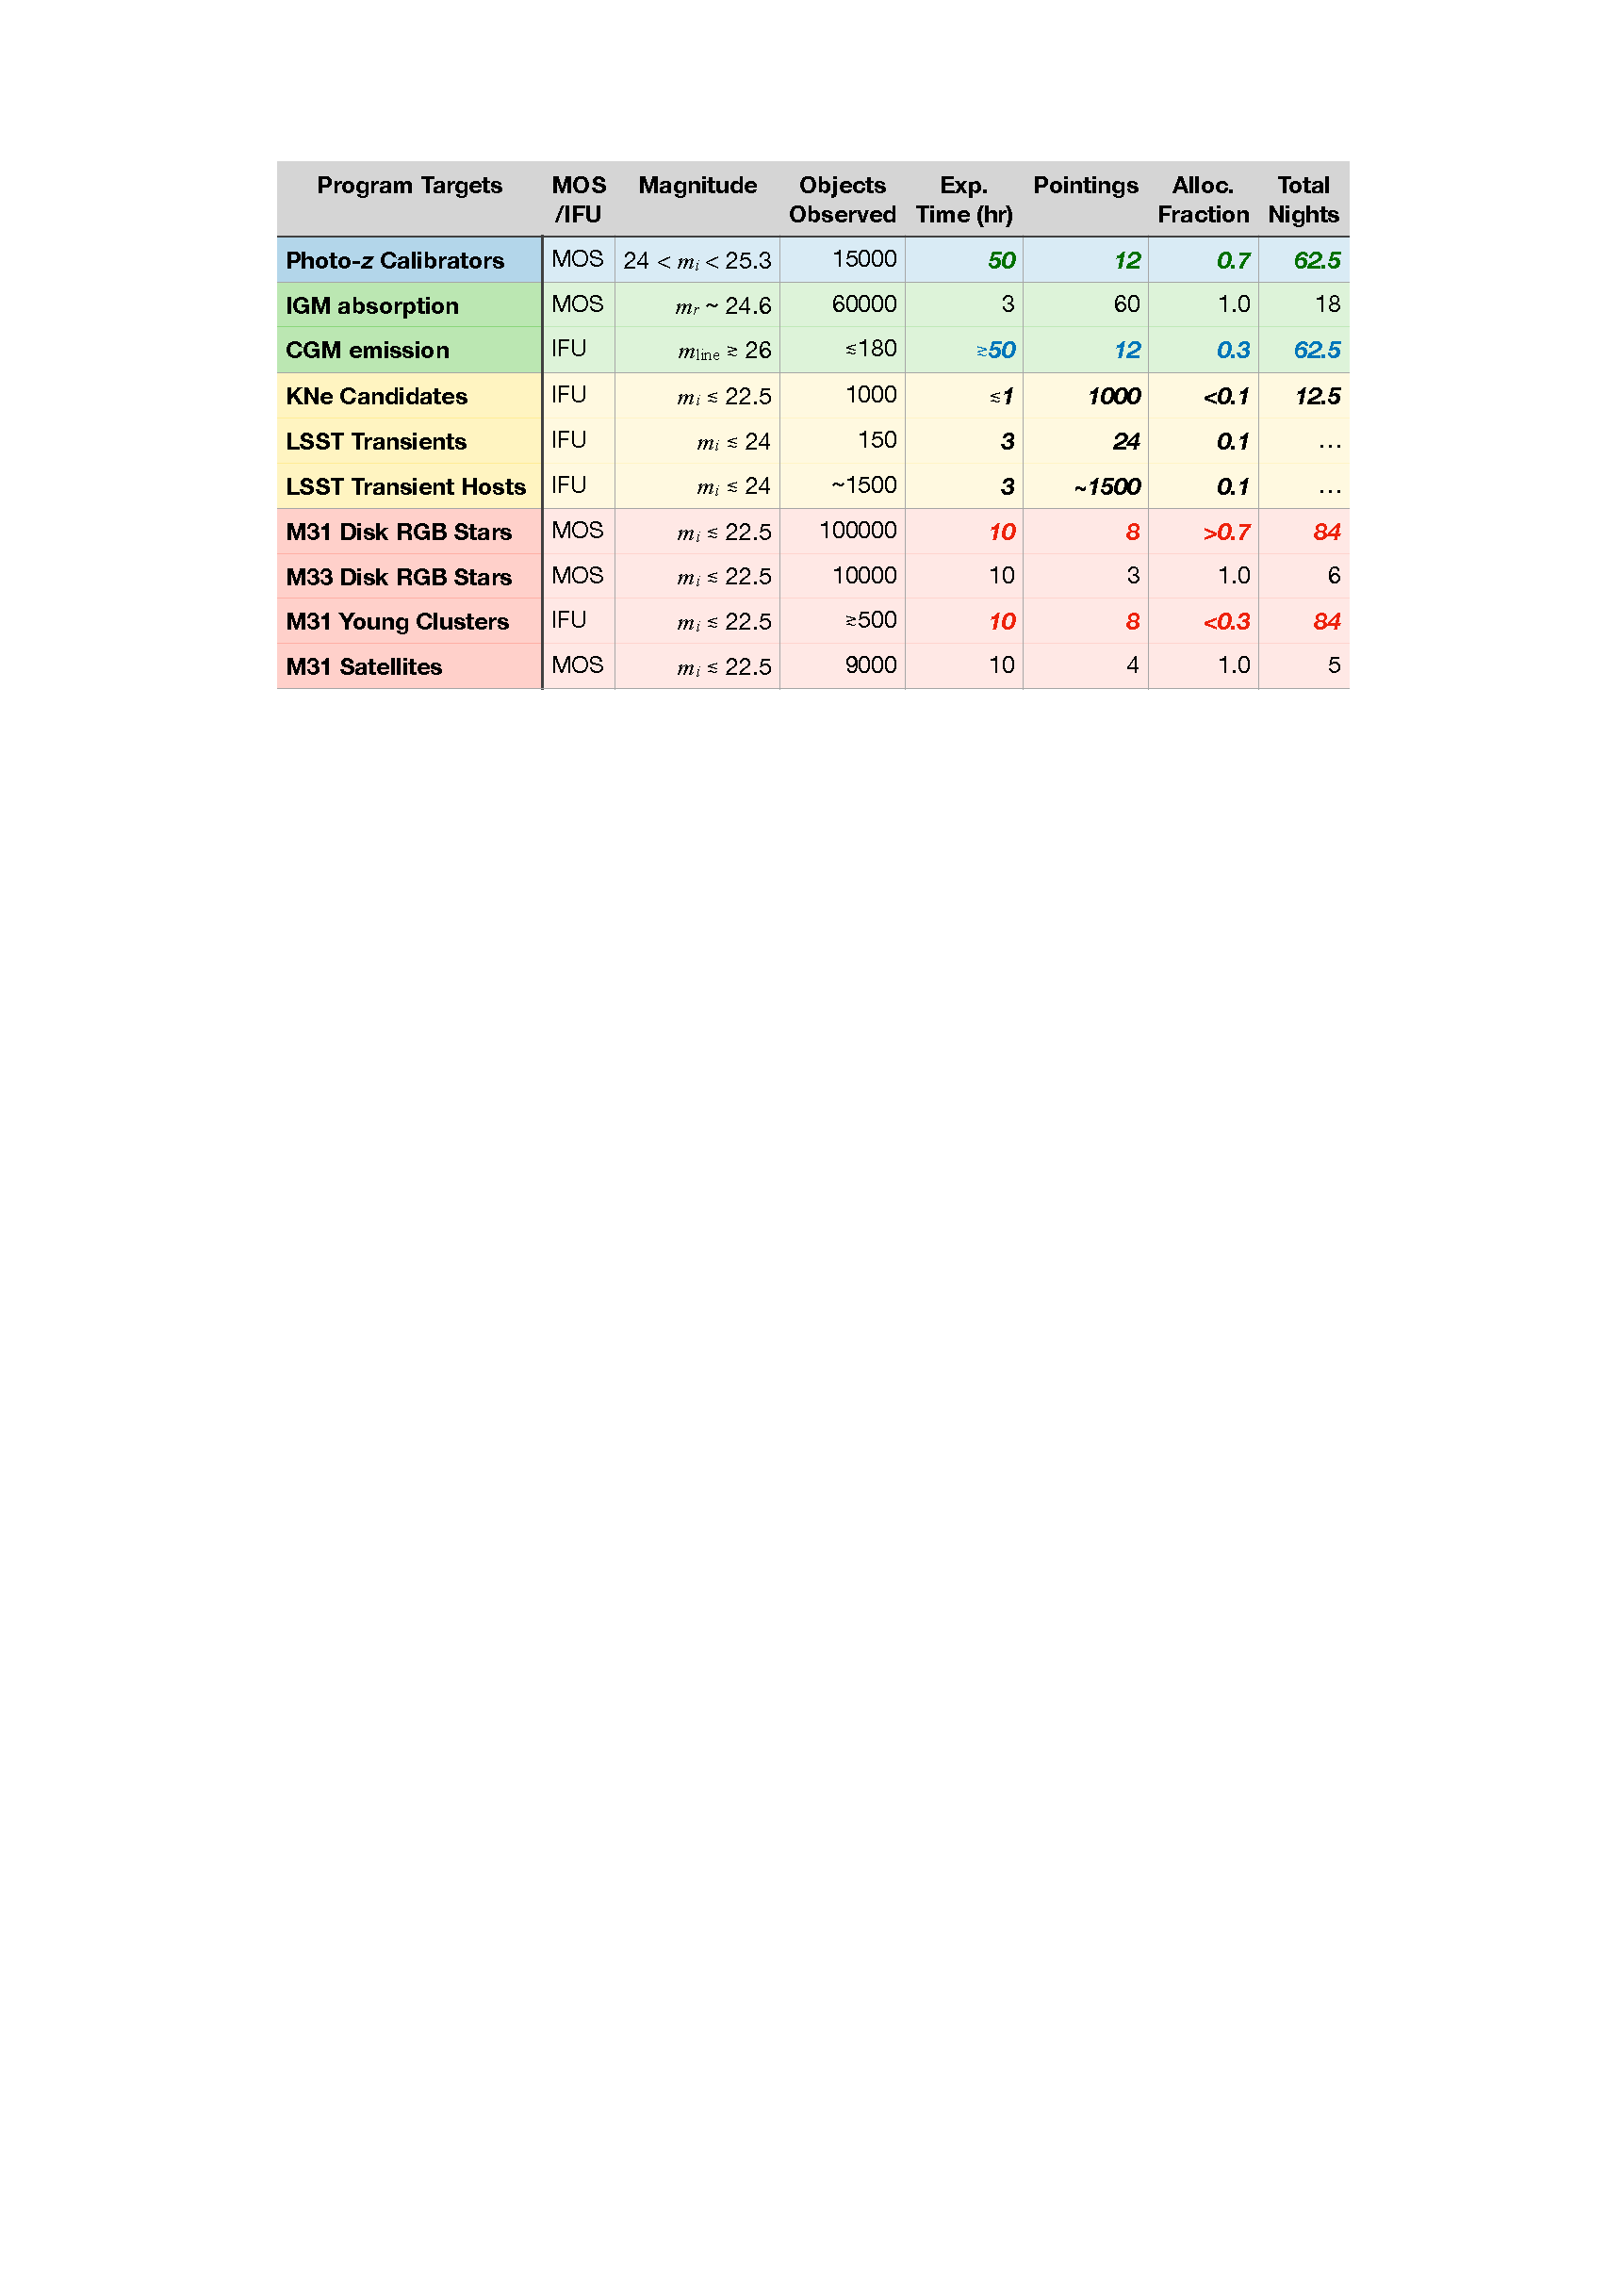
\includegraphics[width=0.85\textwidth]{figs/key_program_summary.pdf}
% \label{tab:progreq}
% \end{figure}

% Serving as both a summary table and an illustration of how FOBOS enables program synergies, Table \ref{tab:progreq} collects salient details for the {\it FOBOS Cosmology} (blue), {\it Galaxy-Ecosystem} (green), {\it Time-Domain} (gold), and {\it Andromeda} (red) Programs.  From left to right, we provide the primary program targets, the required aperture format, the expected source magnitude, the observed sample size, the exposure time per target, the number of unique pointings, the fraction of fibers allocated to the program targets in each configuration, and the total number of nights that would be requested.  Bold entries in the last four columns highlight quantities that are {\it shared} between multiple programs; e.g., observations of photo-$z$ calibrators and CGM emission are completed {\it simultaneously} via a single 62.5-night request. This demonstrates the utility of allocating FOBOS time in terms of ``fiber hours'' given that programs may not require FOBOS's full fiber complement on a given observing night.  Indeed, no nights have been assigned to follow-up of LSST transients or their hosts given that these observations can be integrated with other (e.g., PI-led) observing programs in effectively any FOBOS field.  

% Optimized integration of observing programs is an exciting opportunity in terms of access (as described above), observing efficiency and science return.  It also presents an interesting challenge that the FOBOS team (in particular via our CMU partnership/sub-award) will begin to address during the preliminary design phase.

% \subsection{Deep Learning with FOBOS}
% \label{sec:ML}

% Even with its high target density, FOBOS can never provide spectroscopic follow-up of a significant fraction of targets drawn from upcoming large-scale imaging surveys.  Indeed, {\it billions} of viable galaxy targets will be observable from Keck in the combined LSST, Euclid, and WFIRST photometric catalogs.  A spectroscopic survey of that scale requires techniques still in the early stages of development (e.g., high-throughput photonics).  Fortunately, however, advanced data-analysis methods, adapted from ongoing research in Machine Learning and Statistics, can leverage spectroscopic samples to infer properties of objects with only photometric measurements \citep[e.g.][]{hemmati19}. Recent years have seen significant progress in the development and application of such methods for this purpose; for example, redshift estimation with photometry (``photo-$z$ estimation’’) can now be addressed as a machine-learning problem. While spectroscopic surveys provide the crucial ``training sets’’ required to learn the relationship between colors and redshift, small samples are sufficient in order to build accurate prediction methods, as long as they are representative of the photometric population. Each problem presents unique challenges and requirements, but similar approaches could be taken to infer properties of objects, such as galaxy star-formation rate or stellar age \citep[e.g.][]{TingPayne19}. Hence, a moderate investment in the development of tailored methods of data analysis can yield scientific gains from photometric surveys, comparable to having significantly larger spectroscopic samples.

% With its combination of sensitivity and multiplex, FOBOS on Keck will be ideally suited to such applications in three ways.  First, at least until the advent of 2nd-generation ELT instruments, FOBOS will be unparalleled in its ability to probe the faint end of, e.g., LSST's photometric catalogs. In fact, beyond its immediate application to photo-$z$ training, the 15,000 spectra obtained by the {\it FOBOS Cosmology Program} will serve as an ideal training set for galaxy-evolution studies of the much larger galaxy samples with LSST/Euclid/WFIRST photometry.  Second, FOBOS's ability to collect information (Fig.~\ref{fig:info}) is significantly greater than similar instruments over the same wavelength range.  This allows FOBOS to efficiently build large samples that can be combined with training data of greater depth or higher spectral resolution to, e.g., produce high-level properties of galaxies at high redshift.  Finally, the cost of observing rare targets---critical to constructing training sets that span large volumes of parameter space---is reduced because FOBOS can efficiently combine targets from multiple programs (\S \ref{sec:addsci}).


% \section{Scientific Benefits to the U.S.\ Community}
% \label{sec:community}

% The need for a significant U.S.\ capacity to obtain high-multiplex spectroscopic follow-up in the Rubin era has been
% emphasized in numerous reports.  In 2015, a National Research Council report concluded that ``the National Science
% Foundation should support the development of a wide-field, highly multiplexed spectroscopic capability on a medium- or
% large-aperture telescope...'' \citep{NAP21722}.  A workshop organized by the National Optical Astronomy Observatory in
% 2016 at the NSF's request highlighted specific spectroscopic needs for LSST follow-up in all science areas.  The report
% that followed argued there was an urgent need to ``Develop or obtain access to a highly multiplexed, wide-field optical
% multi-object spectroscopic capability on an 8m-class telescope.''  Our proposal addresses these calls to action.

% Meanwhile, FOBOS also ranks as one of WMKO’s top priorities in the coming decade, as encapsulated in its 2016 Strategic
% Plan and evidenced by WMKO’s commitment to make 30 nights available to the U.S. community over \emph{this MSIP proposal
% period}, thereby deepening community involvement in Keck during the FOBOS design phase.  Relative to this proposal's
% funding request, this 30-night commitment is akin to the return on investment provided by the NSF/NOAO Telescope System
% Instrumentation Program (TSIP) from the last decade.  NSF's NOIRLab will administer these 10 nights of Keck time per
% year from 2021--2023 through the NOIRLab TAC process.

% Looking further ahead, the FOBOS team is actively fostering engagement of the larger U.S.\ community in developing and
% leading future FOBOS public-survey programs of wide scientific benefit. NSF's NOIRLab has agreed to partner with us in
% developing additional ``open-access'' models and building planning tools that, once FOBOS is on-sky, allow U.S.\
% astronomers to propose for a reserved portion of FOBOS fibers. A proposed $\sim$100,000 fiber-hours --- or roughly
% $\sim$160 DEIMOS $+$ $\sim$270 LRIS-B nights --- per year, will allow individual PI programs to be integrated into the
% suite of all FOBOS observations.  NSF's NOIRLab has also agreed to solicit additional key program concepts from the
% U.S.\ community, host workshops on these concepts, and coordinate proposing teams ahead of a competed selection
% process.  The final number of open-access fiber-hours and public survey nights are subject to approval by WMKO, its
% steering committee, and its board.

% DEIMOS nights: 100,000 hr / 100 slits / 6 hours per night = 167 nights
% LRIS nights: 100,000 hr / 60 slits / 6 hours per night = 277 nights

%% \begin{wrapfigure}{r}{0.55\textwidth}%\small
%\begin{figure}
%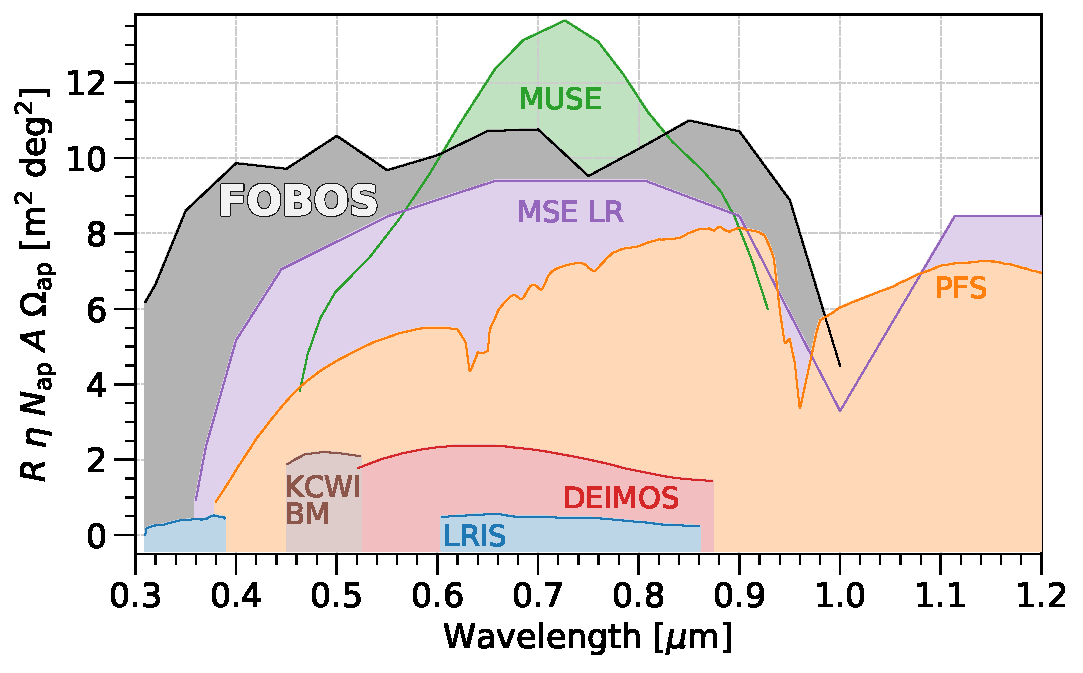
\includegraphics[width=0.55\textwidth]{figs/FOBOS_info_power.pdf}
%\caption{FOBOS's information gathering power relative to a suite of instruments that exist (LRIS, DEIMOS, KCWI, MUSE), are under construction (PFS), or proposed (MSE). For each instrument, we plot the spectral resolution ($R$) times the instrument etendue --- efficiency ($\eta$; ratio of incident to detected photons) $\times$ multiplex ($N_{\rm ap}$) $\times$ telescope effective area ($A$) $\times$ solid angle per aperture ($\Omega_{\rm ap}$).  When photon limited, etendue is inversely propotional to the exposure time required to meet a fixed S/N; we normalize by spectral resolution to reflect the information gathered per angstrom.  Except for VLT-MUSE (a 1\arcmin{}$\times$1\arcmin{} IFU) over 35\% of FOBOS's wavelength range, FOBOS outperforms all other instruments in terms of raw observing power over its spectral range, and it is a factor of 5--10 more powerful than existing optical spectrographs on Keck.  In particular, note the significant difference in blue sensitivity ($\lambda \lesssim 4000 {\rm \AA}$).} 
%\label{fig:info}    
%\end{figure}

% Finally, we have emphasized the design of software platforms necessary
% for a seamless user experience from target submission to data-product
% retrieval and analysis. FOBOS will be the first \emph{general-purpose}
% spectroscopic instrument to automatically provide high-level data
% products such as redshifts, galaxy stellar-continuum fits, emission-line
% properties, and stellar parameters. With a commitment to the public
% release of raw, reduced, and high-level products derived from \emph{all}
% FOBOS observations, these data products will dramatically reduce the
% time from observations to science. Our team has delivered previously in
% this regard, providing the first comprehensive high-level data product
% package for an SDSS survey with MaNGA's\footnote[1]{Mapping Nearby Galaxies
% at Apache Point Observatory (MaNGA) is one of three SDSS-IV core
% programs. Bundy also serves as the MaNGA PI. CoI Westfall led
% development of MaNGA's Data Analysis Pipeline.} Data Analysis Pipeline
% \citep{westfall19} and its interactive public science platform, Marvin
% \citep{cherinka19}.  We will also use our established
% connections\footnote[1]{Co-I Schafer is Co-Chair of Rubin Observatory LSST's ISSC.} to
% LSST's Informatics and Statistics Science Collaboration (ISSC) to
% advertise, recruit, and coordinate efforts on deep-learning tools for
% both key science and FOBOS operations (e.g., our data-driven observing
% optimization tool, MAISTRO, discussed in our Data Management Plan).

%-----------------------------------------------------------------------
%-----------------------------------------------------------------------
\section{Technical Specifications}
\label{sec:project}

\begin{wrapfigure}{r}{0.48\textwidth}
\begin{threeparttable}
\begin{small}
\captionof{table}{Summary of FOBOS Specifications} 
\label{tab:specsummary} 
\begin{tabular}{l | r}
\hline
Telescope                   & 10-m Keck II \\
Patrol Field                 &    $D = 20$\arcmin{} \\
Total Number of Fibers       & 1800 (Table \ref{tab:sampling}) \\
Single-Fiber (MOS) Aperture  &    $D = 0.8$\arcsec{} \\
Multi-IFU FOV (37 fibers)    &    $D = 5.6$\arcsec{} \\
Large IFU FOV (1657 fibers)  &    $D = 37.6$\arcsec{} \\
Spectral Range               &    0.31--1$\mu$m \\
Spectral Resolution          &    3500 \\
Throughput                   &    $\gtrsim$30\% \\
Limiting Magnitude$^\dagger$  &    $r$(AB)$\sim$24.5 \\
\hline
\end{tabular}
\begin{tablenotes}
\item $^\dagger$To reach S/N$\sim$1 in a 1hr integration.
\end{tablenotes}
\end{small}
\end{threeparttable}
\end{wrapfigure}


FOBOS will simultaneously collect spectra from 1800 fibers distributed among single apertures and/or integral-field units (IFUs) across a 20$^\prime$ field.  FOBOS provides deep sensitivity, with $\gtrsim$30\% instrument throughput from 0.31--1.0 $\mu$m, and a spectral resolution of $R \sim 3500$ delivered by three, bench-mounted 4-channel spectrographs (see Table~\ref{tab:specsummary}).  


% \noindent \note{1 page}

% Here's an alternative way to put in figures if we want captions on the side (to save space)
% Could introduce a new ``counter'' to count and label figures appropriately
%\centerline{\hbox{\includegraphics[width=0.6\textwidth, angle=0]{figs/FOBOSatKeck_v1.pdf}
%    \hspace{0.1cm} \vspace{2in}
%    \parbox[b]{0.3\textwidth}{\small {\bf Figure ??:} Rendering of FOBOS instrument systems deployed at the Keck II Nasmyth port.  By mounting the FOBOS spectrographs under the Nasmyth platform, other instruments like DEIMOS can maintain access to the telescope. \vspace{2cm}}}}

\begin{figure}[h!]
\vskip -0.1in
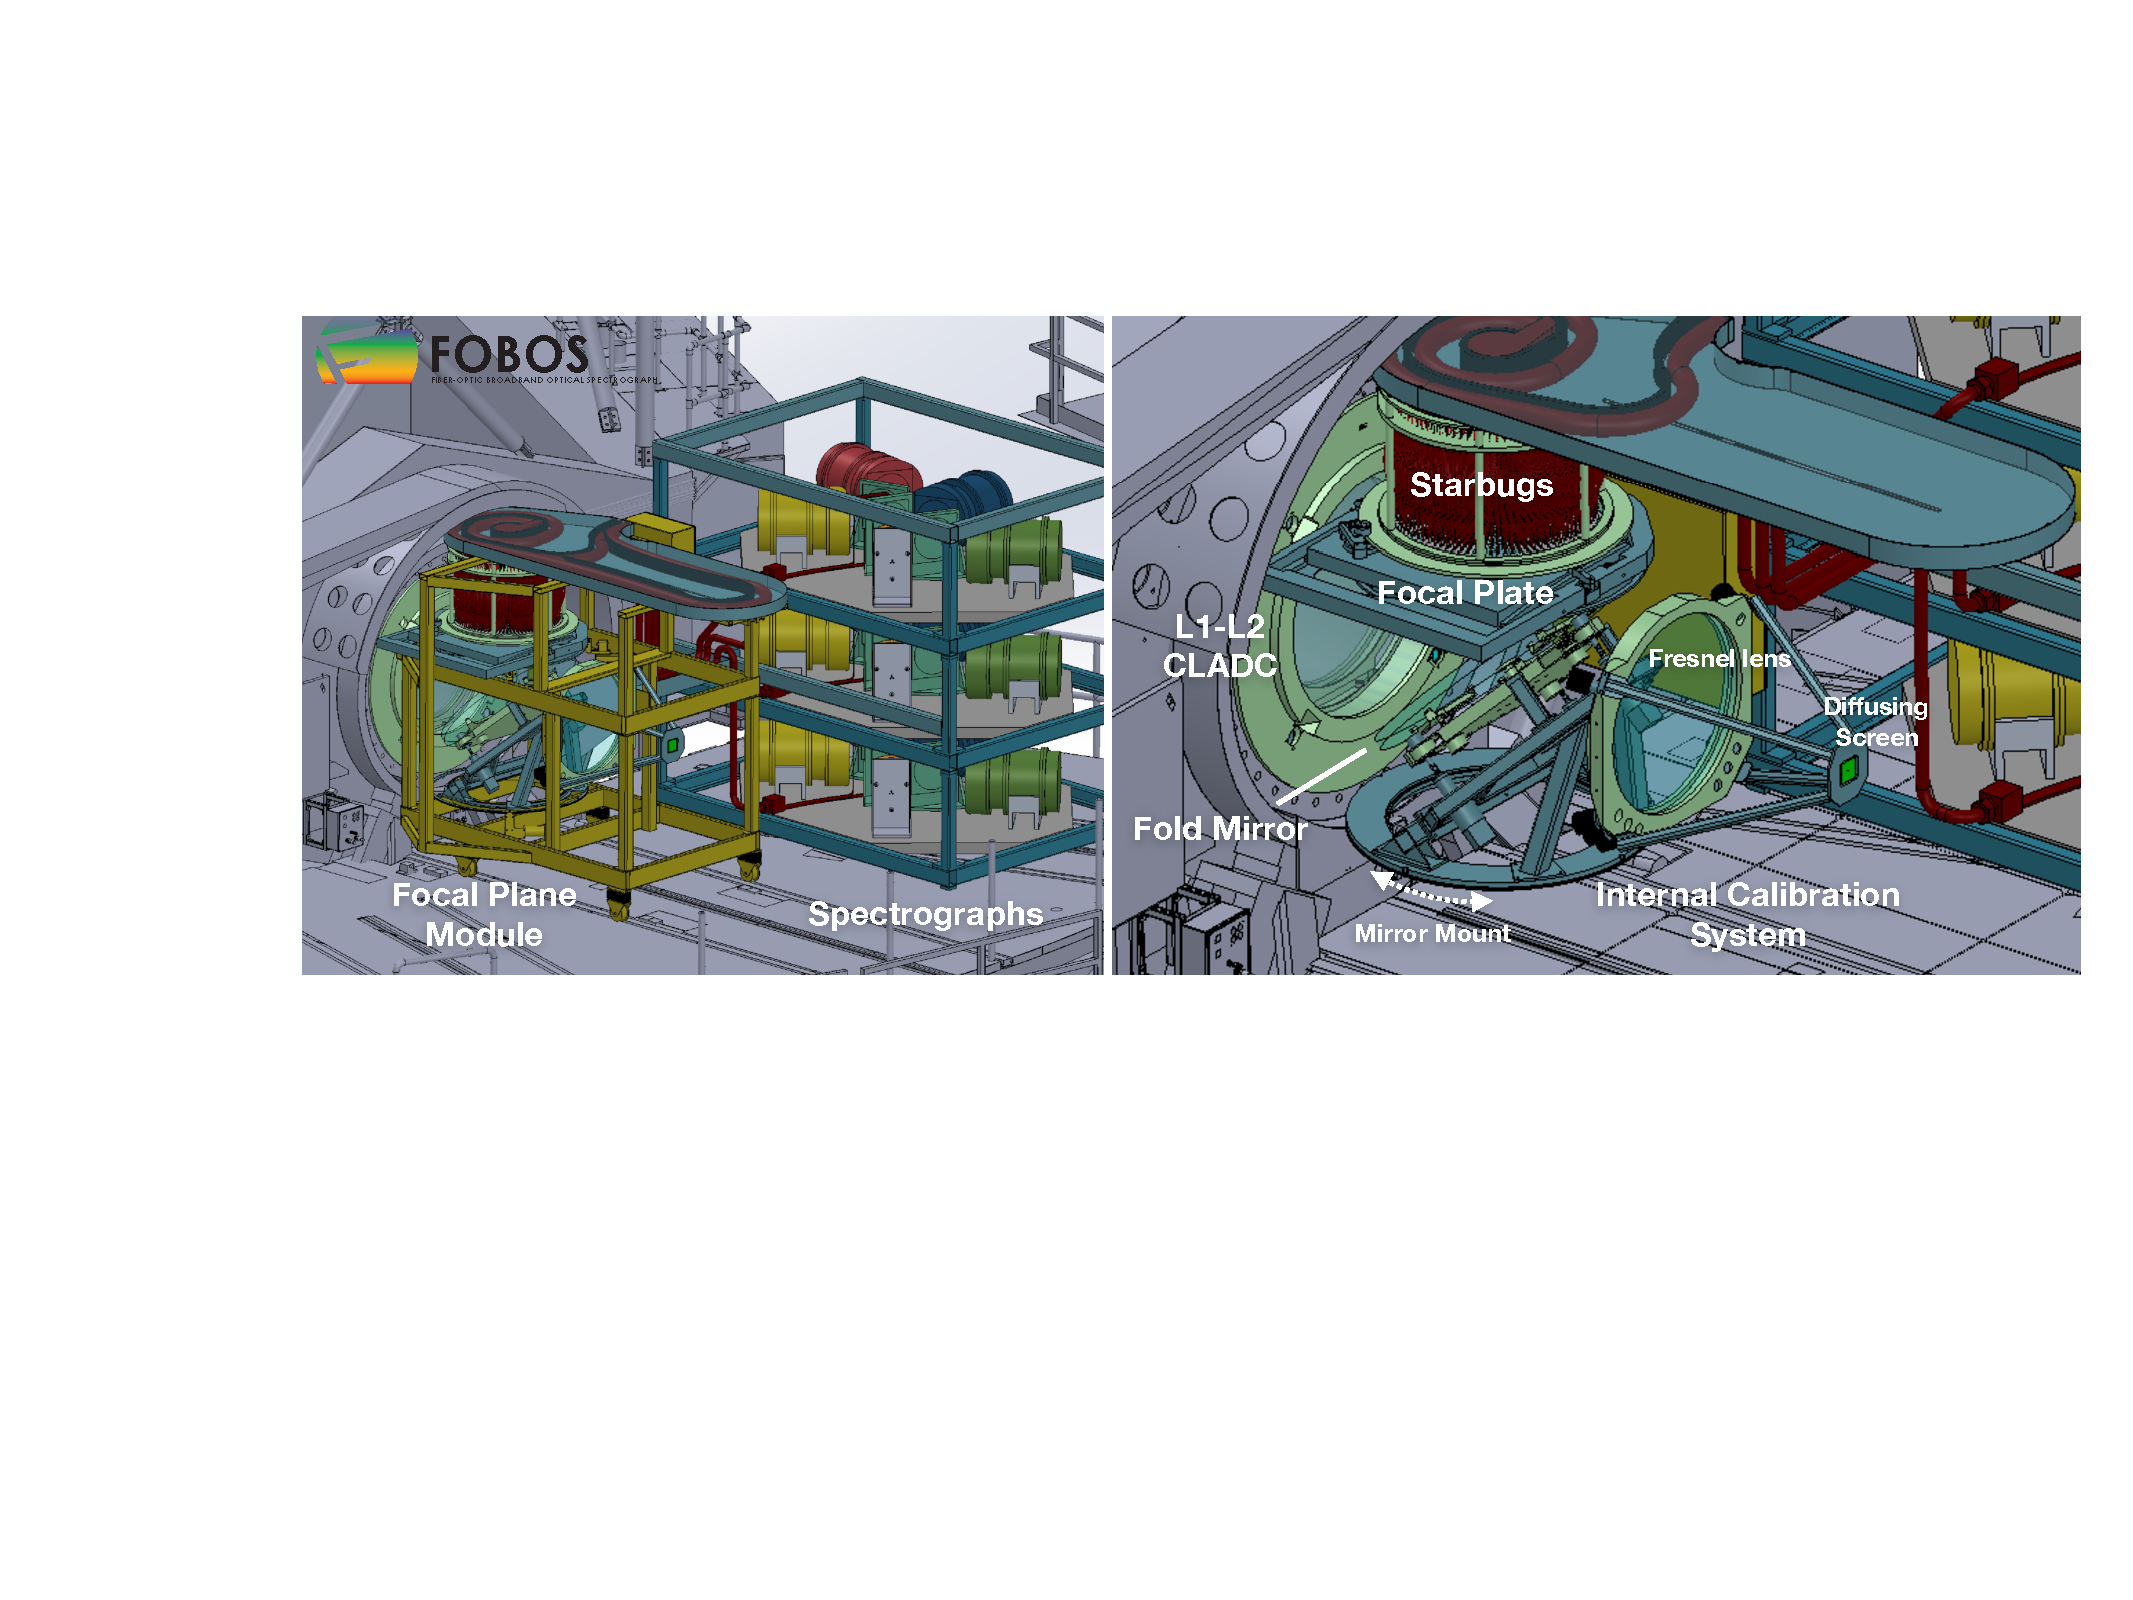
\includegraphics[width=\textwidth]{figs/FOBOS_inst_FPzoom_v2.pdf}
\caption{\small {\it Left}: Rendering of FOBOS instrument systems (without thermal enclosures and electronics packages) deployed at the Keck II Nasmyth port. {\it Right}: Zoom-in of the Focal Plane Module with the support framing removed.}
\label{fig:layout}
\end{figure}

\noindent The current conceptual design of all FOBOS sub-systems are described in the following subsections and summarized in Table \ref{tab:specsummary}.  For each subsystem, we also comment on its technical maturity and heritage, where appropriate.  While grounded in design heritage from previous instruments, FOBOS features several innovations including a horizontal focal plane, the use of Starbugs with either single-fiber or IFU payloads that enable various observing modes, and the use of high-efficiency fused silica etched (FSE) gratings in all spectrograph channels.

\subsection{Focal-Plane Module} The focal-plane module comprises several key systems held in a rolling frame that can be pulled back and stowed, maintaining exchangeable access of multiple instruments to the Keck II Nasmyth port (Fig.~\ref{fig:layout}).  FOBOS's focal-plane module includes the compensating lateral atmospheric dispersion compensator (CLADC), the focal plate and Starbugs positioners, the metrology and calibration systems, and the cable wrap and tray.

\subsubsection{CLADC} The FOBOS CLADC consists of three lenses and a fold mirror, working together to correct the wavelength-dependent angular dispersion caused by the atmosphere when viewing at different zenith angles. The CLADC concept \citep{saunders14} has been adopted for MSE and is under consideration for the GMT.  For FOBOS, the CLADC's fused silica lenses have all-spherical surfaces and diameters of 1.0--1.2 meters.  When FOBOS is deployed, the first two CLADC lenses are positioned slightly ($\sim$200 mm) inside the Nasmyth journal.  The third CLADC lens is at the telescope image plane; it has a curved rear surface to match the curved focal plane and serves as the mounting surface for the Starbug positioners.  The first and third CLADC lenses are articulated by motorized mounts to trace simple arcs.  A field rotator independently rotates the third CLADC lens to track the field angle.

Before converging to the image at the focal plate, the nearly horizontal beam is folded upwards by a 45$^\circ$ mirror before the third lens. This has the substantial benefit of providing a horizontal (i.e., gravity invariant) surface on which the Starbugs roam (see below), but requires an additional 1.6 m of telescope focal length to make room for the fold and focal-plane support structure.  This extended focal length is made possible by a 20 mm shift of the Keck secondary mirror coupled with a slight rephasing of the primary mirror segments (by amounts well within their range of motion) to correct wavefront aberrations to an acceptable level of $\sim$0.3\arcsec{}.  To enable on-board internal calibrations, the fold mirror is able to rotate in the horizontal plane to face away from the telescope and instead accept light from the calibration system.

Zemax modeling shows that the CLADC design delivers superb image quality ($<$0.3\arcsec{} rms diameter) across Keck's entire 20\arcmin{}-diameter unvignetted field-of-view for zenith angles as large as 60$^\circ$, over a bandpass of 350--1000 nm.  The $\sim$6\arcsec{} amplitude of atmospheric dispersion is reduced to $<$0.1\arcsec{}.  Furthermore, the beam's chief ray angles match the surface normal with an average error of 0.06$^\circ$, meeting a conservative 0.1$^\circ$ requirement for negligible geometric focal-ratio degradation.  In the next phase, we will expand the design's bandpass to 310--1000 nm; early analysis suggests excellent performance.  The CLADC is reasonably mature at this design stage, with optical elements well within the fabrication capabilities of several optical suppliers.  The mechanical structure and actuation requirements are low-precision and low-risk.

\subsubsection{Focal-Plane Sampling}

Benefiting from the Starbugs technology (\S \ref{sec:starbugs}), FOBOS has the significant advantage of providing a menu of night-time configurations that allow users to deploy single-fiber apertures (MOS mode), multi-fiber integral-field units (Multi-IFU mode), and combinations thereof.  Fiber connectors enable an exchange, performed during a daytime procedure, between 600 MOS fibers or 15 37-fiber IFUs for each of the three spectrographs.  FOBOS also offers a single large IFU with 1657 fibers (37.6\arcsec{} diameter)
%; Tab.~\ref{tab:specsummary})
that simultaneously feeds all three spectrographs. In practice, portions of the total fiber budget will be allocated to ($\sim$100--200) roaming sky fibers, ($\sim$12) 7-fiber ``mini-bundles'' for flux calibration, and a single 37-fiber IFU (3\arcsec\ in diameter) for rapid-response spectroscopy. Table~\ref{tab:sampling} enumerates the five sampling configurations in the current FOBOS design (note the configuration for combined observations of the {\it FOBOS Cosmology} and {\it CGM Programs} is given in the third row).

% with 1--2\% gap losses between fibers. 

\begin{wrapfigure}{r}{0.4\textwidth}
\begin{threeparttable}
\captionof{table}{FOBOS Sampling Modes$^\dagger$}
\label{tab:sampling}
\begin{tabular}{l | r r }
\hline
Deployed Apertures  & $N_{\rm MOS}$ &  $N_{\rm IFU}$ \\
\hline
Large IFU           &     0 &      1  \\
MOS                 &  1800 &      0  \\
MOS$+$Multi-IFU     &  1200 &     15  \\
MOS$+$Multi-IFU     &   600 &     30  \\
Multi-IFU           &     0 &     45  \\
\hline
\end{tabular}
\begin{footnotesize}
\begin{tablenotes}
\item $^\dagger$Assumes 600 fibers per spectrograph pseudo-slit; detailed apportionment of science, sky, and flux-calibration fibers will be studied in Preliminary Design.
\end{tablenotes}
\end{footnotesize}
\end{threeparttable}
\end{wrapfigure}

Microlens fore-optics coupled to each fiber demagnify and speed up the telescope beam from $f/15$ to $f/5$. This better couples telescope light to the 175 $\mu$m core fiber (${\rm NA} = 0.11$), minimizing losses from geometric focal-ratio degradation (FRD) and providing a maximum effective on-sky diameter of $0.8\arcsec$ per fiber.  Our study of historical Keck seeing measurements (0.67\arcsec\ median over the past 15 years) justifies the choice of 0.8\arcsec\ as a balance between sky noise and aperture loss.
Our IFU designs incorporate 97\%-fill-factor microlens arrays coupled to fiber bundles via fore-optics assemblies.  By deploying different fore-optic designs, 
%versions of the pupil-imaging  fore-optics,
the per-fiber collecting aperture can be reduced while maintaining a fixed fiber core diameter and spectrograph format.  Individual apertures of 0.8\arcsec\ are optimal for our CGM IFU program; however, other IFU programs, to be explored during Preliminary Design, may desire finer spatial sampling of the delivered point-spread function (PSF).

We are currently prototyping microlens optics and optomechanical assemblies for lab and on-sky testing. Lab testing of fiber throughput, output beam profiles, and stress-induced FRD has already begun at both UCO and UCB/SSL.  While we will refine prototyping and process control in our own labs, we are also pursuing commercial options for the full-scale manufacturing of the fore-optics assemblies.

% Optimal fiber aperture trade study here: https://uco.atlassian.net/wiki/spaces/FOB/pages/28606501/Trade+Study+Single-fiber+aperture+size


% \note{From Marc: Note advantages of Starbugs over other zonal positioners.}

\begin{figure}[h!]
\vskip -0.1in
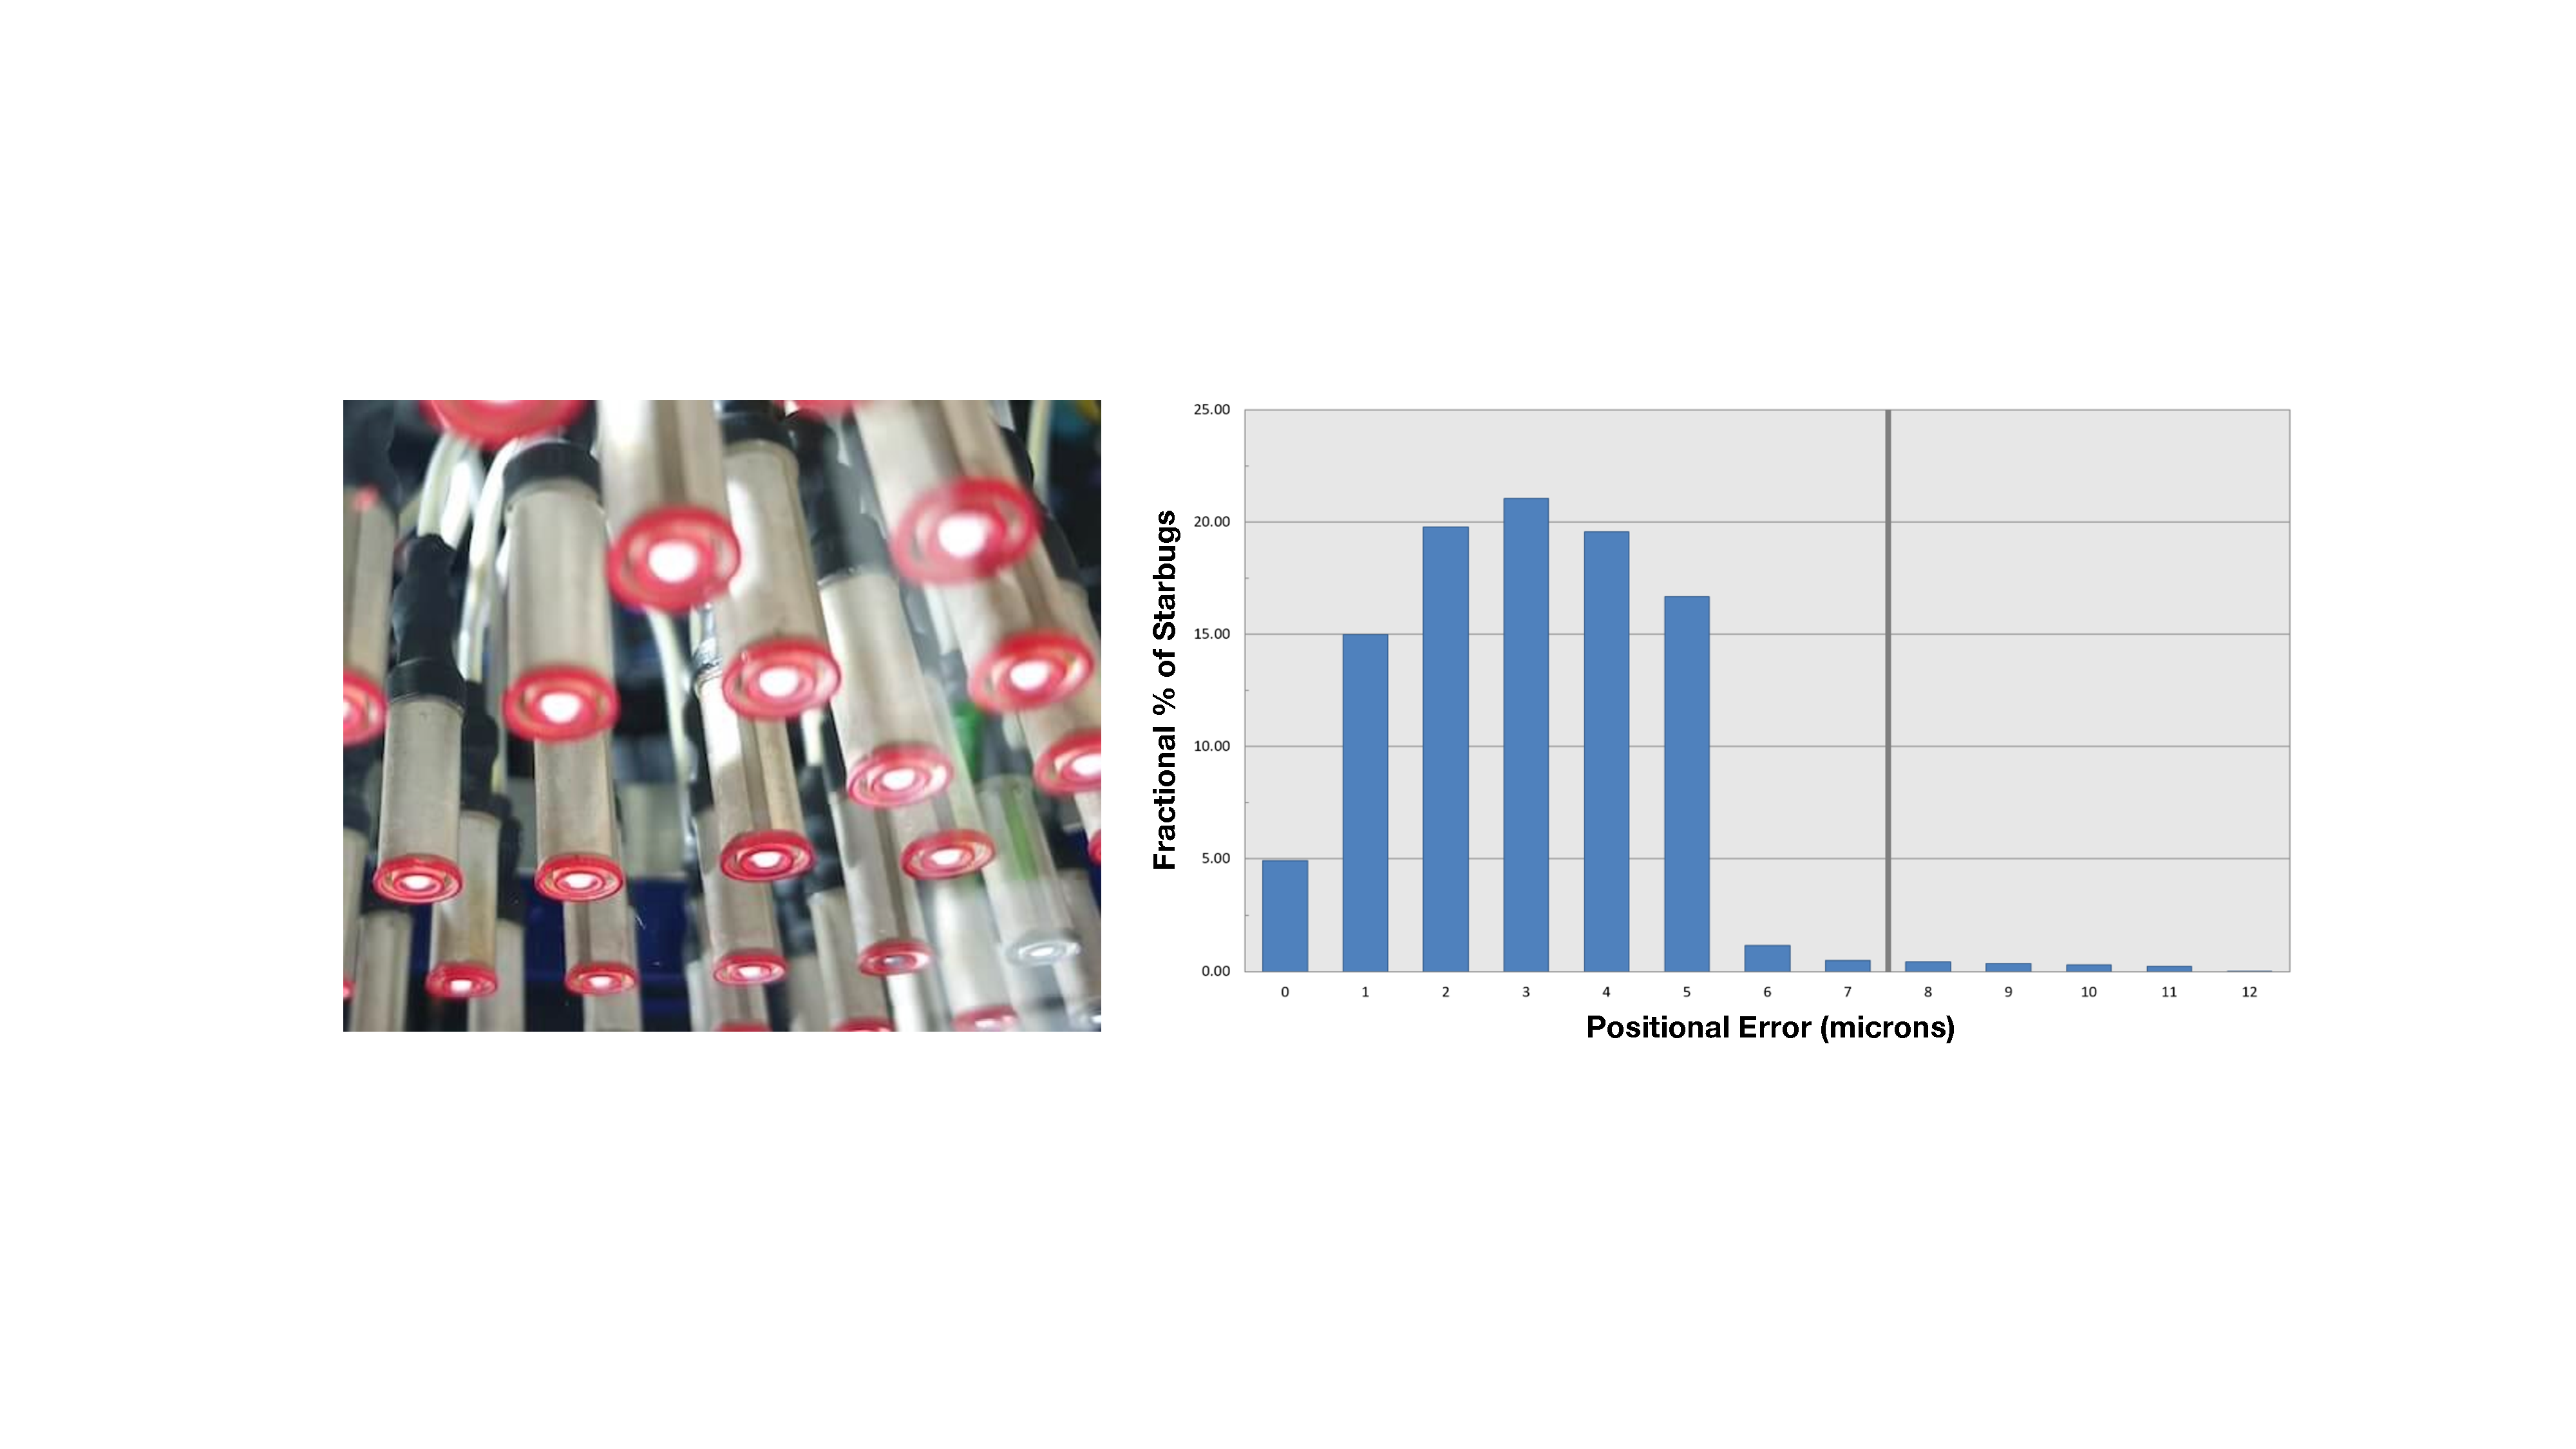
\includegraphics[width=\textwidth]{figs/starbugs_combined.pdf}
\caption{\small {\it Left}: Starbugs fiber positioners depoyed with the TAIPAN instrument. {\it Right}: Distribution of closed-loop positioning accuracy for TAIPAN Starbugs.  An error of $<$7 $\mu$m (vertical line) would correspond to $<$0.01\arcsec{} for FOBOS.}
\label{fig:starbugs}
\end{figure}

%\begin{wrapfigure}{r}{0.30\textwidth}%\small
%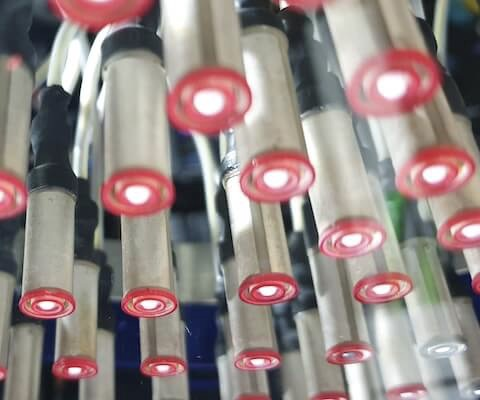
\includegraphics[width=0.30\textwidth]{figs/starbugs_v1.jpg}
%\caption{Starbugs fiber positioners.}
%\label{fig:starbugs}
%\end{wrapfigure}

\subsubsection{Starbugs Robotic Positioners}
\label{sec:starbugs}

FOBOS's flexible focal plane is enabled by Starbug positioners (Fig.~\ref{fig:starbugs}), which unlike fixed-grid zonal positioners, can be deployed with both single-fiber and IFU payloads on the same focal plane.  Starbugs not only allow for multiple observing modes, but have multiple overlapping patrol zones and are efficient for both sparse- and dense-field configurations.  Although switching between deployed modes is currently envisioned to be a daytime procedure, more dynamic, night-time switches will be studied in the next phase.

Starbugs are composed of two concentric cylinders with the payload (single-fiber or IFU) secured in the center. Starbugs can be precisely rotated and ``walked'' across the focal plate using specific high voltage waveforms applied to the piezo actuators of both cylinders. A vacuum seal holds the Starbugs against the plate. FOBOS's horizontal focal plane helps prevent Starbug adhesion loss and allows for smaller, more agile designs that are aided by gravity to stay correctly mounted. Precision positioning is made possible by a metrology system that uses three cameras installed in the support structure of the CLADC to image the bottom face of the focal plate through the fold mirror. Three back-illuminated beacon fibers located in the outer ring of each Starbug allow the system to locate and determine the orientation of each Starbug.

%\begin{wrapfigure}{r}{0.60\textwidth}%\small
%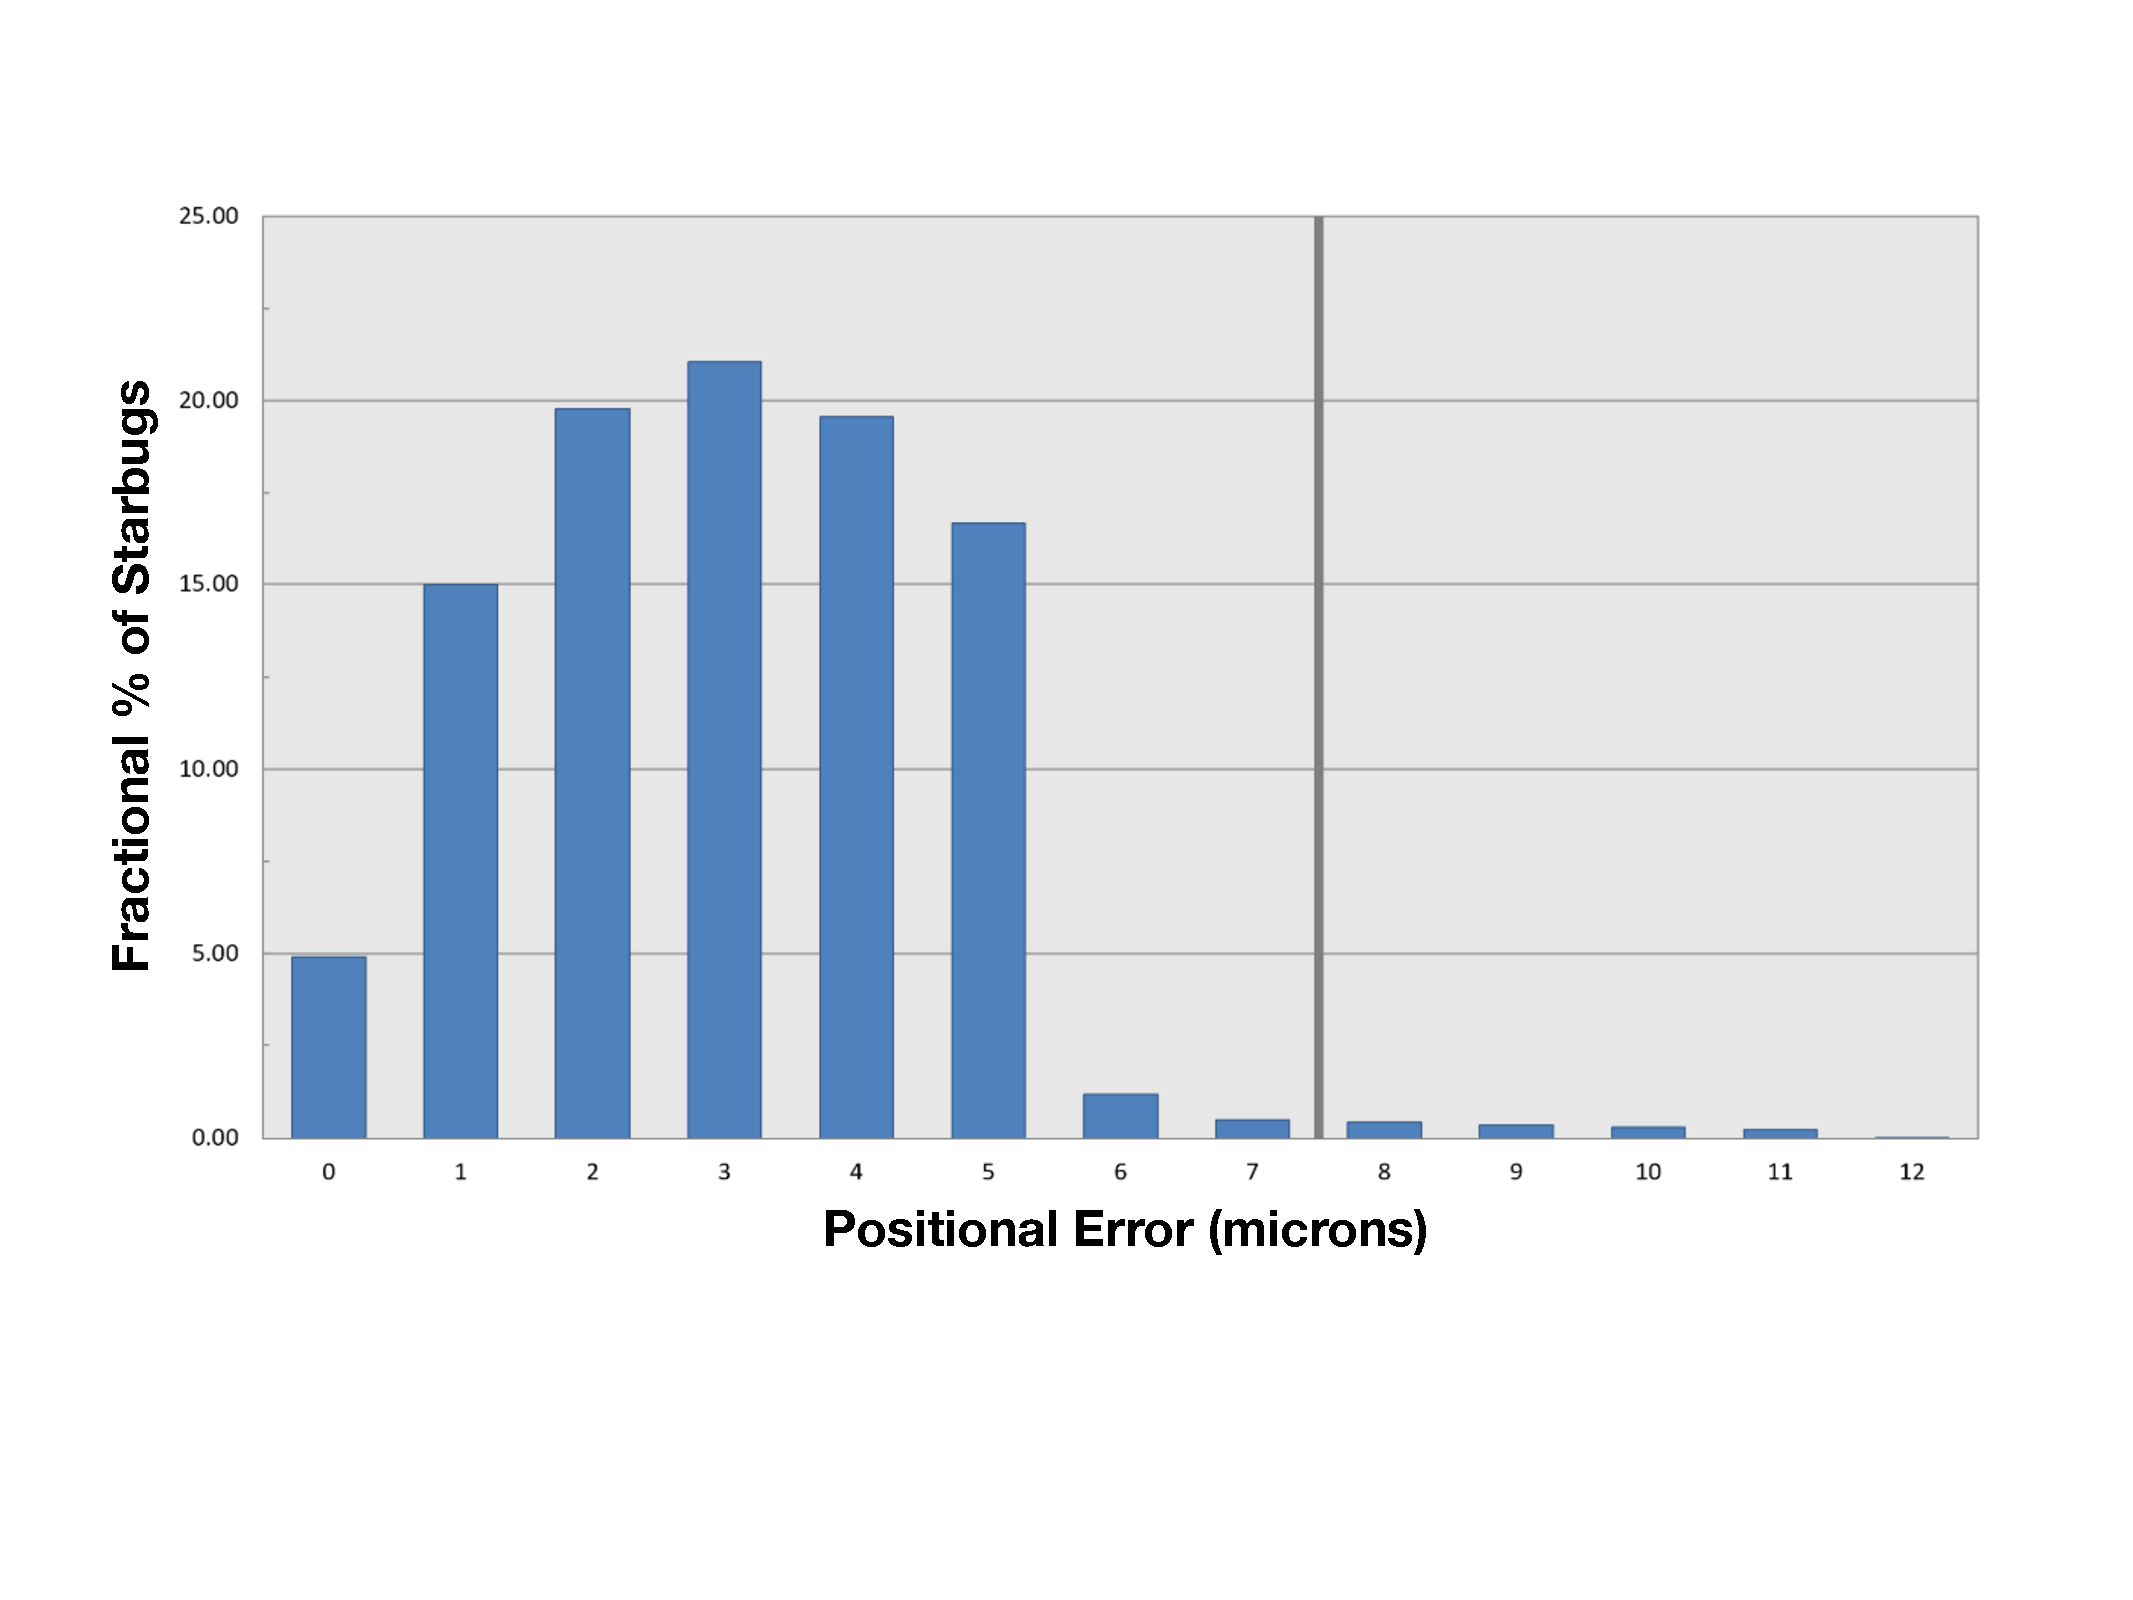
\includegraphics[width=0.59\textwidth]{figs/starbugs_pos_error_v1.pdf}
%\caption{Distribution of closed-loop positioning accuracy for TAIPAN Starbugs.  An error of 7 $\mu$m would correspond to 0.01\arcsec{} for FOBOS.}
%\label{fig:starbugs_error}
%\end{wrapfigure}

Starbugs can patrol regions several arcminutes in diameter and can be placed as close as 10\arcsec{}. The reconfiguration time goal is 2 minutes. AAO\footnote[1]{Australian Astronomical Optics (AAO), formerly Australian Astronomical Observatory.} is currently testing Starbugs on-sky as part of commissioning the TAIPAN instrument,\footnote[1]{TAIPAN, consisting of its fiber-positioning system and spectrograph, deploys 150 Starbugs on the focal plane of the UK Schmidt Telescope at Siding Spring Observatory (NSW, AU).} which has been delayed due to problems unrelated to Starbugs. A number of lessons-learned from the Starbug technology development as part of the TAIPAN instrument are already incorporated into the FOBOS conceptual design.  This experience will also inform our Preliminary Design Phase, including enhanced instrument modularity, ``slipper'' ring design and materials studies, and electronics upgrades.

Starbugs assembly, verification, and test processes have been developed and refined over several years. These tests, along with the data from continuous lifetime tests (equivalent to greater than 5 years of instrument operations), show that only minor and infrequent calibration is needed to maintain successful closed-loop positioning. With a small step size, exquisite positioning accuracy for Starbugs has been demonstrated; positioning accuracy is typically better than 7 $\mu$m for TAIPAN, which is equivalent to 0.01\arcsec{} for FOBOS and well below our requirements  (Fig.~\ref{fig:starbugs}). 
%(Fig.~\ref{fig:starbugs_error}). 

\subsubsection{Fiber Cabling and Stress Relief}

The FOBOS fibr cables will be built following under-sea cable construction techniques; the fibers will be helically wound to allow equal bending, have a central tensile element to prevent stretching, and have a ruggedized sheath for protection. This type of fiber cable construction has been shown to minimize stress-induced FRD, while not restricting the focal-plane motion systems as a result of stiffness.  This method was tested and selected as the cabling system for both PFS and DESI.

\subsubsection{Systematics Control and Calibrations}
\label{sec:calib}

FOBOS is optimized for sensitivity.  We have pursued design choices with a careful eye not only on maximizing throughput but maintaining excellent instrument stability so that exposures can be combined over many nights to build spectroscopic depth.  For the fiber system, we seek minimal stresses and motion, as well as tight angular tolerances at the focal plane and pseudoslit. These should contribute continuum systematics at much less than the 0.1\% level (Bundy et al., in prep).  For the fixed and mounted spectrographs, an enclosure provides temperature control of $\pm 1$C and the refractive-camera designs limit ghosts and scattered light.  Attention to detectors, amplifiers, and electronics is also important.  In addition, our analysis of SDSS-IV/MaNGA data emphasizes the importance of fiber-to-fiber uniformity along the pseudoslit in order to make the instrument response of all fibers (those dedicated to blank sky, calibration targets, or science targets) as similar as possible.  

The importance of precise calibrations for FOBOS has motivated a comprehensive strategy that combines daytime dome-screen observations with nighttime ``internal'' calibrations at regular intervals.\footnote[1]{Keck does not support dome calibrations at night.}  In the afternoon, flat-field and arc-line exposures are first taken through the telescope of a carefully-illuminated interior dome screen.  This provides the ``true'' instrument flat-field and wavelength solution.  Internal calibrations are then taken by rotating the fold mirror to accept light from a ``pupil-injection'' system included in the focal-plane module (Fig.~\ref{fig:layout}).  This secondary calibration system includes separate lamps, a structure diffuser screen, and a 1 m diameter commercial Fresnel lens that act to mimic the telescope pupil.  While not designed to be as flat as the dome-screen observations, the secondary calibration will be \emph{stable}.  Reference to the simultaneous dome-screen calibration can be used to solve for a ``flat'' internal calibration.  At night, changes in instrument stability owing to temperature or fiber state can be corrected through regular internal calibration exposures, as often as hourly, depending on the observing program's requirements.  Use of the sky background through a model of the instrument$+$sky$+$calibration response provides a final step in the calibration process.  High flux densities will be achieved with the calibration sources, enabling useful exposure times of $\sim$10 seconds.  Thus, internal calibrations can be completed in 2--5 minutes and automated to occur, e.g., during telescope slews, to reduce overheads.

% Do we want a short paragraph concerning sky subtraction?  I.e, what does the above buy us assuming 100-200 sky fibers?

In most observing modes, FOBOS will deploy $\sim$12 7-fiber ``mini-bundles'' to observe Milky Way F sub-dwarfs in the field-of-view appropriate for simultaneous spectrophotometric ``flux'' calibration \citep{yan16}.  Accounting for both transparency and PSF-induced aperture losses, this method will provide a relative flux precision of 3--5\% across the FOBOS wavelength range in routine observations.
%, as demonstrated by existing instruments.

\begin{figure}[h!]
\vskip -0.1in
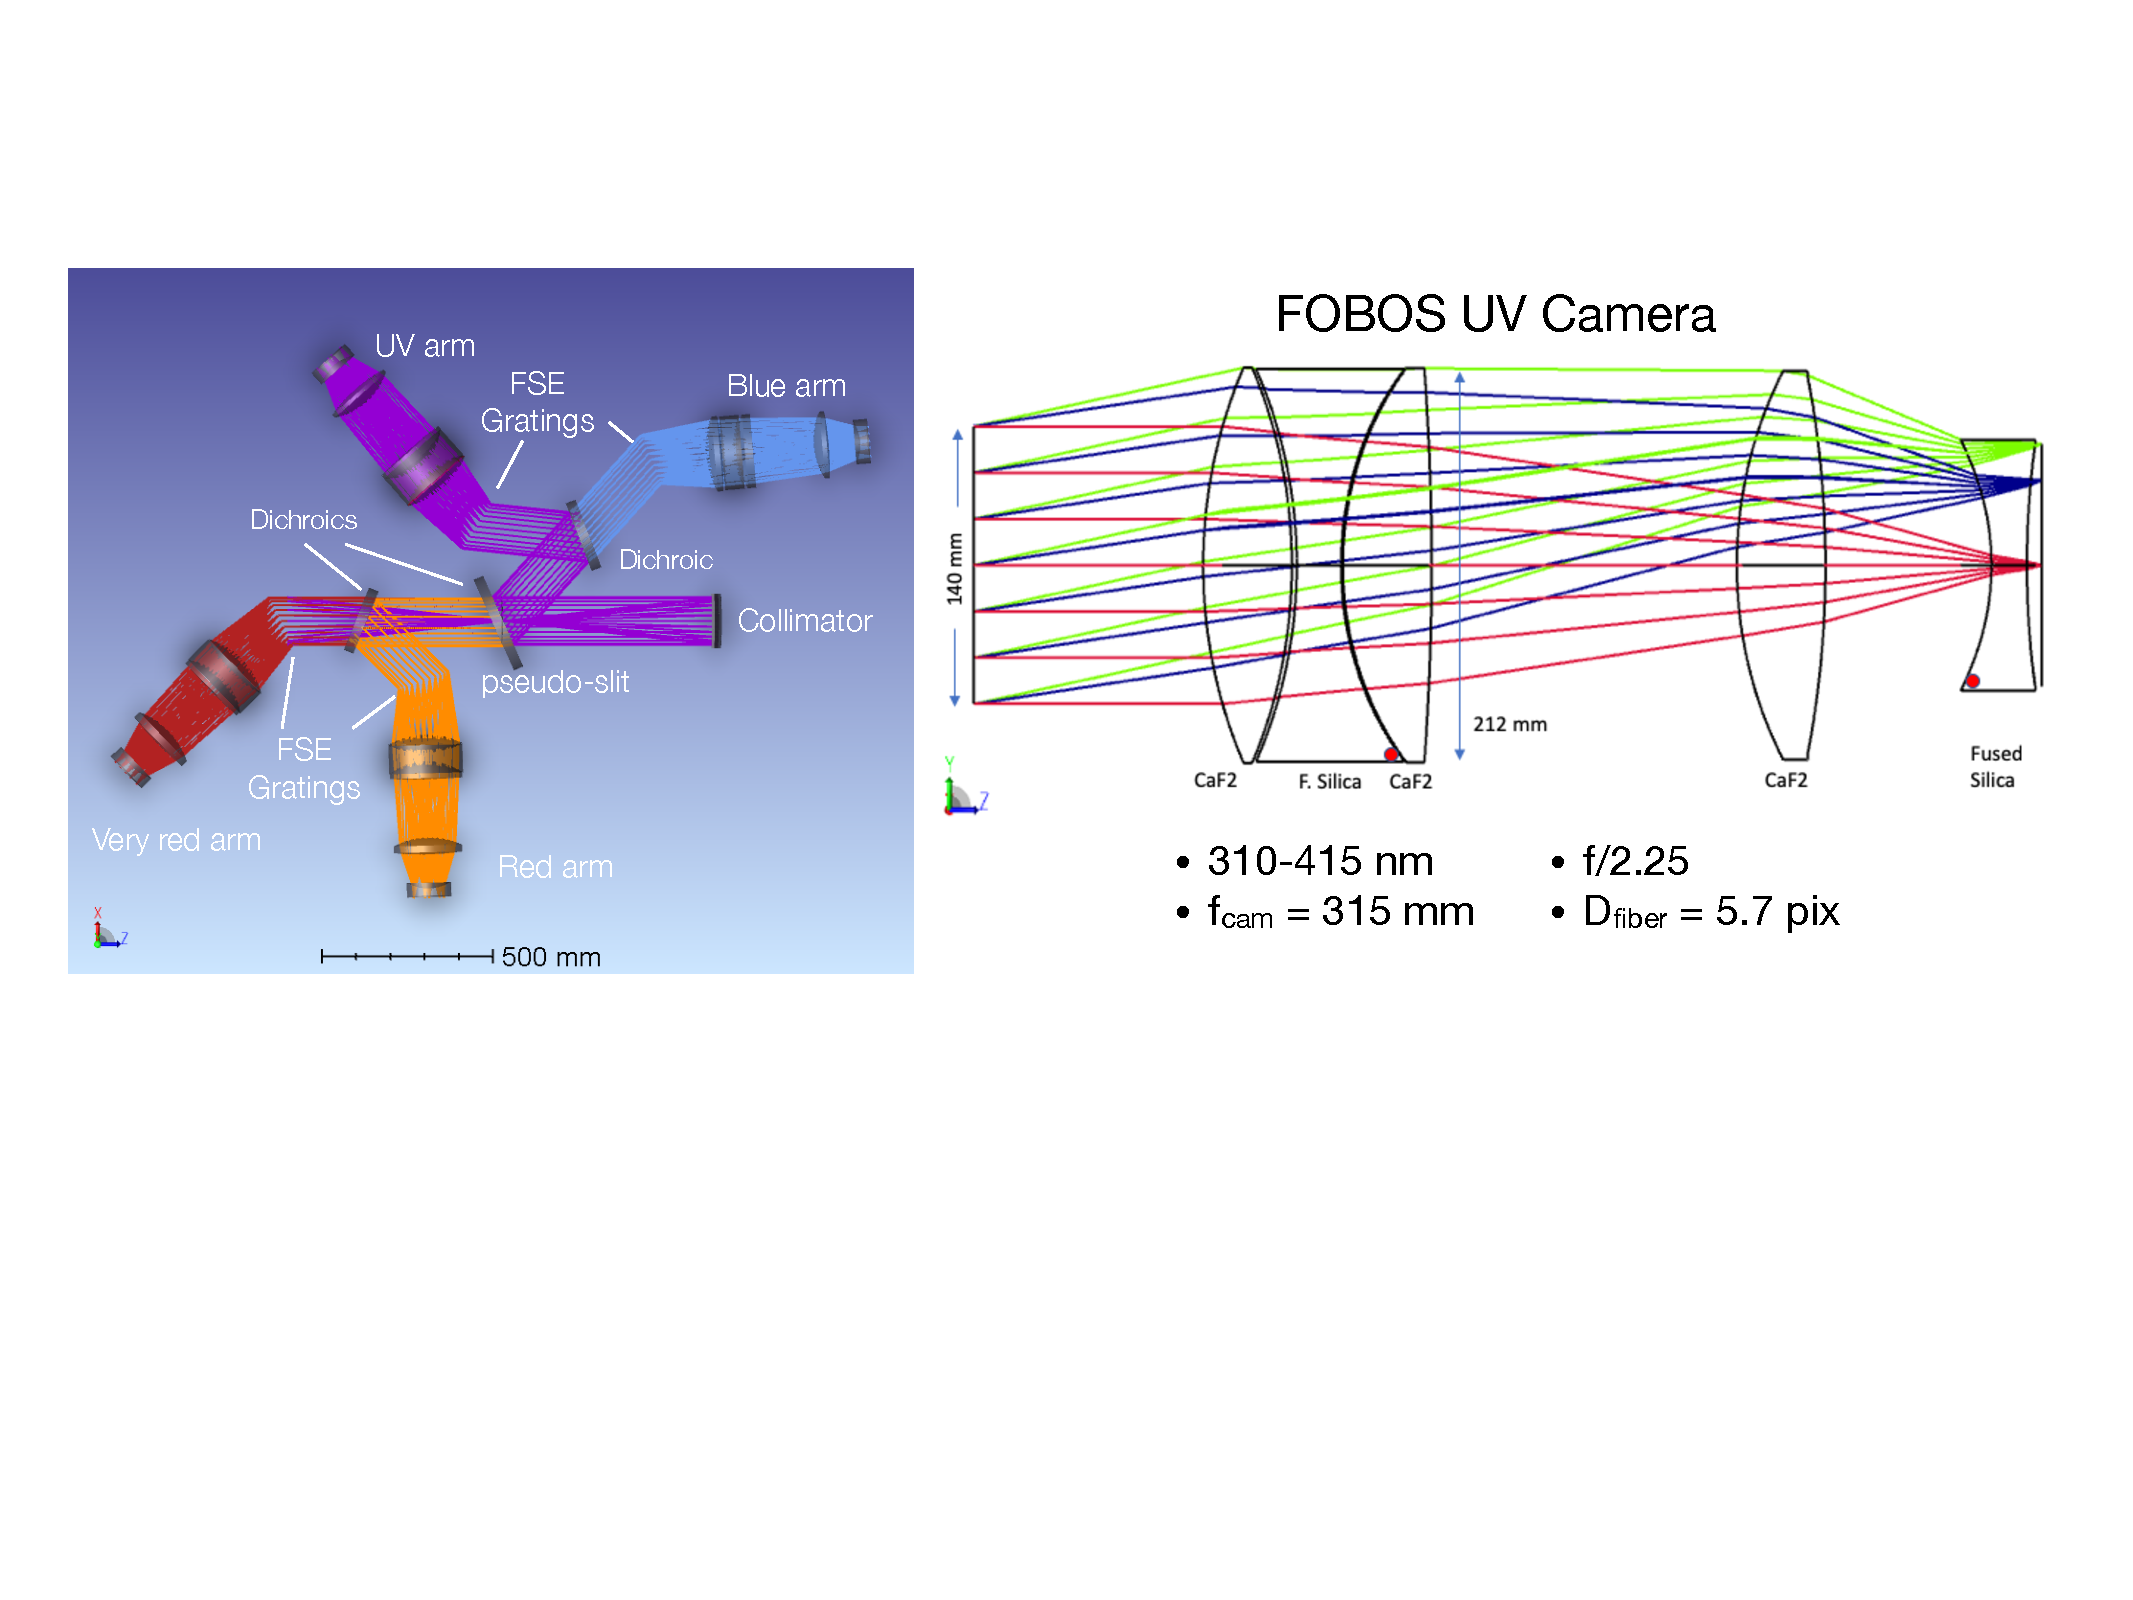
\includegraphics[width=\textwidth]{figs/Spec_and_UVcam_v1.pdf}
\caption{\small {\it Left}: Spectrograph optical design. {\it Right}: UV channel camera design.}
\label{fig:spec}
\end{figure}

\subsection{Spectrographs}

FOBOS employs three identical spectrographs mounted adjacent to the focal-plane module on the Keck II Nasmyth deck and fed by a short ($<$15 m) fiber run in order to preserve UV throughput.  Each spectrograph accepts 600 fibers with 175 $\mu$m core diameter and ${\rm NA} = 0.11$.  Fibers are glued into v-groove blocks mounted on in-beam pseudoslits.  The expanding output beam strikes a collimating mirror with $F_{\rm coll} = 630$ mm. A series of dichroics divide the 140 mm diameter collimated beam into four wavelength channels with a combined, instantaneous spectral range of 0.31--1 $\mu$m. High-efficiency fused-silica etched (FSE) gratings \citep{ZeitnerFSE} provide mid-channel spectral resolutions of $R \sim 3500$.  Each channel employs f/2.25 refractive cameras with $F_{\rm cam} = 315$ mm using designs based on the optical prescription of the f/1.7 DESI cameras and optimized for the channel’s bandwidth.  For the bluest wavelength channel (310--415 nm), the DESI design and glass choice has been modified for performance at these UV wavelengths (Fig.~\ref{fig:spec}).  Using 6k$\times$6k CCDs with 15 $\mu$m pixels for each channel, the demagnified diameter of a monochromatic fiber spot is sampled by 5.7 pixels. Taking advantage of the fixed spectral format, our design makes use of anti-reflective detector coatings applied with a spatial gradient to optimize performance at the wavelength associated with each CCD row. With on-chip binning that modestly oversamples the monochromatic fiber spot, we expect exposures to be background limited at the blue edge of FOBOS's spectral range with a 10-min integration.

% We don't talk about vendors at all, but interesting question from John Wilson: "Regarding the DESI cameras, is there any requirement, perhaps due to intellectual property rights, that FOBOS cameras will need to be fabricated by Winlight?"

The spectrographs are mounted in a permanent temperature-controlled housing, providing a stable environmental temperature ($\pm$1C). Heat rejection of electronics components in the dome is done through a glycol cooling loop. Cyrogenic cooling of the science detectors will be provided by liquid N$_2$ (LN2) or closed-cycle coolers. The estimated end-to-end instrument throughput peaks at 60\% and is greater than 30\% over 95\% of the combined bandpass.

\subsection{Upgrade Paths}
\label{sec:upgrades}

FOBOS's ability to easily deploy and exchange different fiber collectors on the focal plane opens exciting upgrade paths.  These include deploying fibers feeding future spectrographs, e.g., with $R \sim 20,000$ spectral resolution or near-IR sensitivity, to the FOBOS focal plane.   Another is taking advantage of ground-layer adaptive optics (GLAO) corrections from an anticipated GLAO system at Keck II. GLAO improves depth, enables crowded source targeting, and opens new science territory through spatially-resolved galaxies beyond $z\sim0.5$. Particularly for the latter, we would expect to deploy an IFU mode that critically sampled the improved GLAO PSF.


% \noindent \textbf{Data Management System.} FOBOS requires a robust software suite 
% to handle observational planning, data collection, processing, and serving. An API (Application Programming Interface)
% communicates between the following major sub-systems. {\it The Doctor}: A database of metadata and performance metrics,
% as well as analysis software, to monitor instrument health and predict performance. {\it The Producer}: Planning,
% simulation, and execution of integrated, multiple-pointing observing programs based on {\it MAISTRO}\footnote[1]{MAISTRO:
% Modular Artificial Intelligence System for Target Reallocation and Observing.}, an ``artificial intelligence'' (AI)
% targeting system that will learn optimization strategies for user-controlled and multi-program target assignment. {\it The Accountant}: A data-reduction pipeline with
% runtime options for both quick-look and science-ready reductions. {\it The Alchemist}: Automated derivation of
% high-level data products (e.g., redshifts). {\it The Curator}: An archive of all data and data products as well as a
% dynamic interface and science platform for visualization and analysis.  \note{All: Now that we have to provide a separate document for this, can we remove this section and just reference the Data Management Plan here and/or somewhere else in the text; e.g., Section 2?}
% 
% \note{Yuan-Sen: currently, myself included, there is a strong interest to also merge The Doctor with The Producer, i.e., forecasting seeing using time series metadata. The same for The Accountant/Alchemist. With automated quick analysis pipeline, one could adjust S/N requirement and exposure on the fly. I wonder if we should expand our imagination of AI beyond The Producer. Basically, most of these can be wrapped under AI and optimized over (and it is really not that far fetch).} 

% \noindent \textbf{MAISTRO: Target Allocation with Artificial Intelligence} Powered by Starbugs fiber positioners, FOBOS will enable fast, dynamic
% reallocation of fibers.  To efficiently determine the best options given
% a wide range of possible targets and desired observing outcomes, we will
% develop a preliminary design for MAISTRO\footnote[1]{MAISTRO: Modular
% Artificial Intelligence System for Target Reallocation and Observing.}
% an ``artificial intelligence'' (AI) targeting system that will learn
% optimization strategies for assigning targets from a database of
% overlapping observing programs with pre-defined priorities.  The AI
% package will aggregate data quality using a quick-look reduction
% package, science-driven performance metrics, {\it and real-time
% assessments of the observing conditions} to make dynamic targeting
% recommendations.  For example, if conditions are slightly less than
% optimal, MAISTRO would reconfigure Starbugs to brighter objects in a
% field or implement a different program prioritization.  MAISTRO will
% incorporate updated target lists and priorities from the active observer
% and could easily be over-ridden at any time.   Fractions of the full
% FOBOS multiplex might also be reserved ``manual targeting'' as required
% by the program PI.  

%   - maintains a database with observational progress on individual
%     targets in the survey and
%   - dynamically reallocates fibers based on real-time assessments of
%     the aggregate S/N of each target to meet the specific need of each
%     science case.

% This requires significant design and testing of a combined software
% package and hardware interface.  Specific considerations involve (1)
% fast and robust reduction procedures (cf. MaNGA DOS) that can assess
% the aggregate data and (2) a responsive database with a schema
% optimized for real-time decision making to select targets for
% (re)acquisition while accounting for collision limitations.  Provided
% enough design effort, this lends itself to a machine-learning
% application.


% \setcounter{page}{1}
\bibliographystyle{spiebib}
%\bibliographystyle{jponew.bst}
\bibliography{references}

\end{document}


